% RLJ main.tex Version 2025.0

\documentclass[10pt]{article}
\usepackage[accepted]{tmlr} 

\def\month{10}  % 2-digit month for camera-ready version
\def\year{2026} % 4-digit year for camera-ready version
\def\openreview{\url{https://openreview.net/forum?id=VrWIwB8g3Z}}

\usepackage{amsmath}
\usepackage{amssymb}           
\usepackage{mathtools}         
\usepackage{mathrsfs} 
\usepackage{graphicx}      
\usepackage{subcaption}         
\usepackage{url}                
\usepackage{amsthm} 
\usepackage{thmtools}
\usepackage{algorithm, algpseudocode}
\usepackage{bbm}
\usepackage{booktabs}
\usepackage{enumitem}
\usepackage{microtype}

\usepackage[pagebackref=false,breaklinks=true,colorlinks=true,linkcolor=blue,citecolor=blue,urlcolor=blue]{hyperref}

\def\N{\mathbb{N}}
\def\R{\mathbb{R}}
\newtheorem{assumption}{Assumption}
\newtheorem{fact}{Fact}
\newtheorem{lem}{Lemma}
\newtheorem{defn}{Definition}
\newtheorem{thm}{Theorem}

\newcommand{\Yb}{\mathbf{Y}}
\newcommand{\Xb}{\mathbf{X}}


\newcommand{\beqan}{\begin{eqnarray*}}
\newcommand{\eeqan}{\end{eqnarray*}}

\newcommand{\beqa}{\begin{eqnarray}}
\newcommand{\eeqa}{\end{eqnarray}}

\def\environment{\mathcal{E}}
\def\environments{\Theta}
\def\proxy{\tilde{\environment}}
\def\target{\chi}
\def\agent{\mathcal{G}}
\def\agents{\Gamma}
\def\data{\mathcal{D}}
\def\actions{\mathcal{A}}
\def\policies{\mathcal{P}}
\def\observations{\mathcal{O}}
\def\hist{\mathcal{H}_{t}}
\def\nonterminal{\overline{\mathcal{H}}}
\def\states{\mathcal{S}}
\def\aggs{\mathcal{X}}
\def\loss{\mathcal{L}}
\def\Regret{{\rm Regret}}
\def\KL{\texttt{KL}}
\def\Hel{\mathbf{d}_{\mathrm{H}}}
\def\Was{\mathbf{d}_{\mathrm{W}}}
\def\TV{\mathbf{d}_{\mathrm{TV}}}
\def\E{\mathbb{E}}
\def\Pr{\mathbb{P}}
\def\I{\mathbb{I}}
\def\H{\mathbb{H}}


\newcommand{\KLp}{\mathbf{\tilde{d}}_{\textrm{KL}}}
\newcommand{\X}{\mathcal{X}}
\newcommand{\Y}{\mathcal{Y}}
\newcommand{\D}{\mathcal{D}}
\newcommand{\A}{\mathcal{A}}
\newcommand{\Prob}{\mathbb{P}}
\newcommand{\argmax}{\mathop{\mathrm{argmax}}}

\newcommand{\Dir}{\texttt{Dir}}
\newcommand{\DP}{\texttt{DP}}

\newcommand{\bH}{{\mathbb{H}}}


\title{Bayesian Neural Networks via Dirichlet Process Priors on the Data-Generating Distribution for Randomized Value Functions in Deep Reinforcement Learning}

%\setrunningtitle{Bayesian neural networks with Dirichlet process %priors for reinforcement learning}


\author{\name Sumit Vashishtha \email vash.sumit@gmail.com \\
      \addr Independent Researcher
    }

% The \author macro works with any number of authors. Use \AND 
% to separate the names and addresses of multiple authors.

\newcommand{\fix}{\marginpar{FIX}}
\newcommand{\new}{\marginpar{NEW}}

\def\month{10}  % Insert correct month for camera-ready version
\def\year{2026} % Insert correct year for camera-ready version
\def\openreview{\url{https://openreview.net/forum?id=VrWIwB8g3Z}} % Insert correct link to OpenReview for camera-ready version





%%%%%%%%%%%%%%%%%%%%%%%%%%%%%%%%%%%%%%%%%%%%%%%%%%%%%%%%%%%%%%%%
%% Begin document, create title and abstract
%%%%%%%%%%%%%%%%%%%%%%%%%%%%%%%%%%%%%%%%%%%%%%%%%%%%%%%%%%%%%%%%
\begin{document}

%\makeCover  % Create the cover page
{\maketitle} % Make the title section

\begin{abstract}
Bayesian neural networks (BNNs) offer a principled framework for quantifying epistemic uncertainty. However, standard weight-space priors yield complex, high-dimensional neural network posteriors that are computationally prohibitive to sample from, and popular approximate inference schemes often fail to capture epistemic uncertainty effectively---a failure mode particularly acute in reinforcement learning (RL) \citep{osband2018randomized}. To resolve this challenge, we introduce a new class of BNNs that quantify uncertainty by placing Bayesian nonparametric Dirichlet Process (DP) priors directly on the underlying data-generating distribution rather than on network parameters. Building on this foundation, we develop DP-DQN, a reinforcement learning algorithm that leverages DP-BNNs to maintain posterior distributions over value functions and perform efficient Thompson sampling. By grounding randomized value functions in Bayesian nonparametrics, DP-DQN unifies data-driven posterior reweighting (via the Bayesian Bootstrap) with prior beliefs and stochastic optimism injected directly through the DP base measure, enabling decisive ``deep exploration'' with a single neural network without the overhead of multi-network ensembles.
\end{abstract}



\section{Introduction}

A fundamental aspect of Reinforcement Learning (RL) is the exploration-exploitation dilemma: in order to maximize cumulative reward, agents need to trade off what is expected to be best at the moment (exploitation) with potentially sub-optimal exploratory actions. Solving this trade-off efficiently to maximize cumulative reward is a significant challenge as it requires reliable uncertainty estimates. Furthermore, exploratory actions should be coordinated throughout extended multi-step decision sequences---a property known as \emph{deep exploration}---rather than selected independently at each individual state.

\textit{Thompson Sampling} \citep{thompson1933likelihood, russo2018tutorial, riquelme2018deep} provides an elegant approach that tackles the exploration-exploitation dilemma by maintaining a posterior distribution over models and selecting actions in proportion to the probability that they are optimal. While these models are conventionally drawn from parametric distribution families (e.g., exponential families), Thompson sampling can in principle be applied to any statistical model admitting tractable posterior sampling \citep{riquelme2018deep}. A natural choice for such statistical models is Bayesian Neural Networks (BNNs), owing to their universal function approximation and rich representation learning capabilities. In contrast to standard neural networks that provide only point estimates, a BNN specifies a prior distribution over parameters $\theta$. Given $n$ training observations $z_{1:n}$, one infers a posterior distribution over $\theta$, which in turn captures epistemic uncertainty in function predictions.

In deep RL, one can represent value functions with BNNs and drive exploration via Thompson sampling over value-function predictions. However, exact posterior inference over neural network weights is notoriously intractable, prompting extensive research into approximate Bayesian methods. These range from Monte-Carlo (MC) dropout \citep{gal2016dropout} and variational inference \citep{blundell2015weight} to stochastic mini-batch Markov Chain Monte Carlo \citep{neal2012bayesian}. Unfortunately, deep RL algorithms built on these weight-space approximate Bayesian methods struggle on hard-exploration tasks because they fail to capture function-space epistemic uncertainty faithfully \citep{osband2018randomized}. This deficiency stems largely from the difficulty of designing meaningful priors directly in parameter space \citep{arbel2023primer}: while practitioners frequently possess domain knowledge regarding the data-generating process (e.g., transition dynamics and reward scales), mapping such insight into high-dimensional, isotropic parameter priors on millions of coupled weights $\theta$ is rarely straightforward and often causes posterior uncertainty collapse.

To resolve these limitations, we introduce a new class of BNNs that quantify epistemic uncertainty by placing Bayesian nonparametric Dirichlet Process (DP) priors directly on the underlying data-generating distribution rather than on network parameters. Notably, posterior inference under a DP prior decomposes naturally into two complementary components \citep{vashishtha2026bayesian, vashishtha2025leveraging}: a data-driven reweighting of observed experience (the Bayesian Bootstrap) and an explicit prior base measure. When transferred to reinforcement learning, this decomposition allows randomized value functions to combine the empirical adaptability of bootstrap ensembles \citep{osband2016deep} with a principled Bayesian mechanism for injecting prior beliefs and stochastic optimism. Crucially, while previous methods require training and maintaining an ensemble of separate neural networks to preserve diversity \citep{osband2018randomized}, our Dirichlet Process formulation achieves targeted deep exploration within a \emph{single neural network}.

We summarize our primary contributions as follows:
\begin{itemize}
    \item We introduce Bayesian Neural Networks with Dirichlet Process priors (DP-BNNs), a paradigm that captures predictive uncertainty by treating the underlying data-generating distribution as an infinite-dimensional random measure governed by a DP prior. Using the Sethuraman stick-breaking construction, we develop a practical sampling scheme for DP-BNNs and validate its epistemic uncertainty quantification against established Bayesian benchmarks on toy datasets.
    
    \item We develop DP-DQN, a deep reinforcement learning algorithm that represents action-value functions via DP-BNNs to perform efficient Thompson sampling. We show that DP-BNNs capture value-function uncertainty through two coherent mechanisms: (i) nonparametrically reweighting transitions in the replay buffer via the Bayesian Bootstrap, and (ii) injecting stochastic optimism into unexplored regions through the DP base measure.
    
    \item We demonstrate that DP-DQN successfully drives deep exploration on challenging benchmarks including RiverSwim and DeepSea (scaling up to depth $N=50$), achieving exploration efficiency competitive with multi-network bootstrap ensembles while operating with a single living network and eliminating multi-head parameter storage.
\end{itemize}

The remainder of this paper is organized as follows. Section~\ref{sec:related-works} discusses related work. Section~\ref{sec:Background-DP} reviews Dirichlet Processes and their stick-breaking construction. Section~\ref{sec:DP-BNNs} presents DP-BNNs alongside epistemic uncertainty benchmarks. Section~\ref{sec:DP-BNN-randomized-value-functions} introduces DP-DQN and evaluates its exploration capabilities. Section~\ref{sec:conclusions} concludes with directions for future work.


\section{Related Works}
\label{sec:related-works}

\paragraph{Randomized Value Functions and Exploration in Deep RL.}
Our work connects directly to deep reinforcement learning algorithms that explore via randomized value functions, replacing heuristic $\epsilon$-greedy exploration with principled posterior sampling (Thompson Sampling) \citep{thompson1933likelihood, osband2016deep, russo2018tutorial}. In deep RL, the most direct approach to Thompson sampling is to maintain a Bayesian neural network over action-values. However, exact posterior inference over network weights is intractable \citep{mackay2003information}, and mini-batch MCMC schemes scale poorly to online RL loops \citep{welling2011bayesian}. Consequently, practitioners have relied on approximate inference methods such as Monte-Carlo dropout \citep{gal2016dropout} and mean-field variational inference \citep{blundell2015weight}. Unfortunately, these weight-space approximations fail to maintain sufficient function-space diversity in unvisited regions, leading to severe exploration collapse in challenging environments \citep{osband2018randomized}.

\paragraph{Bootstrap Ensembles and Prior Mechanisms.}
To preserve functional diversity without exact weight posteriors, \citet{osband2016deep} introduced Bootstrapped DQN, which approximates posterior sampling using an ensemble of $K$ neural networks trained on nonparametrically resampled data. In sparse-reward deep exploration tasks, however, unconstrained bootstrap ensembles collapse because all heads predict identical default values on unseen states. To enforce persistent optimism, \citet{osband2018randomized} introduced Bootstrapped DQN with Randomized Prior Functions (BootDQN-RP), adding a fixed, randomly initialized neural network $p_k$ to each trainable head $f_{\theta_k}$. While empirically effective, this approach is heuristic and substantially inflates computational and memory overhead by maintaining an ensemble of $K$ separate neural networks, each paired with an untrainable prior network. Another approach, Bayesian Deep Q-Networks (BDQN) \citep{azizzadenesheli2018efficient}, applies Bayesian linear regression to the final layer representations; however, its capability on deep-exploration benchmarks has remained largely unexplored in the literature, and our empirical evaluations on DeepSea show that BDQN fails to solve the task. This outcome is not surprising, as restricting Bayesian inference strictly to the final linear readout cannot compensate for the lack of epistemic uncertainty in the underlying deep feature representations on unvisited states.

\paragraph{Bayesian Nonparametrics and Data-Space Priors.}
In contrast to prior works that either operate in parameter space \citep{blundell2015weight} or rely on ad-hoc additive network ensembles \citep{osband2018randomized}, our approach formulates uncertainty nonparametrically directly in data space. By placing a Dirichlet Process prior on the data-generating distribution, DP-BNNs bridge Rubin's classical Bayesian Bootstrap \citep{rubin1981bayesian}---which corresponds to the non-informative limiting case $\alpha \to 0$---with a fully principled prior base measure $F_0$. As we show, the DP base measure naturally injects prior knowledge and stochastic optimism without requiring additive frozen networks or multi-model ensembles, enabling true deep exploration with a single living network at minimal computational overhead beyond standard DQN \citep{mnih2015human}.



\section{Background on Dirichlet Processes}
\label{sec:Background-DP}

This section reviews essential foundational concepts regarding Dirichlet Processes, conjugate posteriors, the Bayesian Bootstrap, and stick-breaking representations that underpin our DP-BNN framework.

\paragraph{Dirichlet distribution.}
The Dirichlet distribution is a multivariate generalization of the Beta distribution. We denote the Dirichlet distribution parameterized by $(\alpha_{1}, \dots, \alpha_{n})$ as $\Dir(\alpha_{1}, \dots, \alpha_{n})$, whose probability density function is given by:
\begin{equation}
p(w_1, \dots, w_n) = \frac{\Gamma(\sum_{i=1}^{n}\alpha_i)}{\prod_{i=1}^{n}\Gamma(\alpha_i)} \prod_{i=1}^{n}w_{i}^{\alpha_i-1}
\end{equation}
for $(w_{1}, \dots, w_{n}) \in [0,1]^{n}$ lying on the simplex $\sum_{i=1}^{n}w_{i} = 1$.

\paragraph{Dirichlet Processes.}
In the Bayesian formalism, an unknown object of interest is treated as a random variable endowed with a prior distribution. When the unknown object is itself a probability measure on a measurable space $(\Theta, \mathcal{B})$ (e.g., a Polish space endowed with its Borel $\sigma$-algebra), defining a prior over infinite-dimensional distributions while satisfying unit-measure normalization is challenging. \citet{ferguson1973bayesian} introduced the \emph{Dirichlet Process} (DP)---a distribution over probability measures that induces finite-dimensional Dirichlet distributions on partitions. Concretely, a random probability measure $G$ is Dirichlet Process distributed with base probability measure $F_0$ and concentration parameter $\alpha \in \mathbb{R}^{+}$, denoted $G \sim \DP(\alpha, F_0)$, if for every finite measurable partition $(A_1, \dots, A_r)$ of $\Theta$:
\begin{equation}
(G(A_1), \dots, G(A_r)) \sim \Dir(\alpha F_0(A_1), \dots, \alpha F_0(A_r)).
\end{equation}

\paragraph{Conjugacy and Posteriors.}
For parametric models, posterior distributions are typically obtained via Bayes' theorem. In nonparametrics, posterior inference over infinite-dimensional measures is generally intractable and relies on conjugate prior families. A family of priors $\mathcal{Q}$ is conjugate with respect to an observation model if the posterior under any prior $Q \in \mathcal{Q}$ belongs to $\mathcal{Q}$. The Dirichlet Process is conjugate to independent identically distributed sampling \citep{ferguson1973bayesian}. Specifically, let $X_1, \dots, X_n \in \Theta$ be independent observations drawn from an unknown distribution $G \sim \DP(\alpha, F_0)$. The posterior distribution of $G$ given $\mathbf{X}_n = (X_1, \dots, X_n)$ is itself a Dirichlet Process:
\begin{equation} \label{def:DP-posteriors}
G \mid \mathbf{X}_n \sim \DP(\alpha_n, \overline{F}_n), \quad \text{where} \quad \alpha_n = \alpha + n, \quad \overline{F}_n = \frac{n}{\alpha+n}{F}_n + \frac{\alpha}{\alpha+n}F_0,
\end{equation}
where $F_n(x) = \frac{1}{n}\sum_{i=1}^{n}\mathbb{I}(X_{i} \le x)$ denotes the empirical distribution of the observations \citep{ghosal2010dirichlet}.

Notice how the posterior base measure $\overline{F}_n$ in Equation~\eqref{def:DP-posteriors} naturally balances empirical evidence $F_n$ with prior structure $F_0$. As sample size $n \to \infty$, the empirical data dominates; conversely, when data is scarce ($n \to 0$), the prior $F_0$ governs.

\paragraph{Bayesian Bootstrap.}
The Bayesian Bootstrap \citep{rubin1981bayesian} provides a Bayesian analogue to Efron's classical bootstrap \citep{efron1994introduction}. Crucially, the Bayesian Bootstrap arises as the non-informative limiting case of a Dirichlet Process posterior as the prior concentration vanishes, $\alpha \to 0$ \citep{ghosal2017fundamentals}:
\begin{equation}\label{def:Bayesian-Bootstrap}
\mathrm{BB}_n := \lim_{\alpha \to 0} \DP\left(\alpha + n, \, \frac{n}{\alpha+n}F_n + \frac{\alpha}{\alpha+n}F_0\right) = \sum_{i=1}^{n} W_{i}\delta_{X_{i}},
\end{equation}
where $\mathbf{W}_n = (W_{1}, \dots, W_{n}) \sim \Dir(1, \dots, 1)$ and $\delta_{X_i}$ denotes a Dirac measure at observation $X_i$. The posterior mean of any linear functional under the Bayesian Bootstrap evaluates simply as $\mu(\mathrm{BB}_n) = \sum_{i=1}^{n} W_{i} X_{i} = \langle \mathbf{W}_n, \mathbf{X}_n \rangle$.

\paragraph{Stick-Breaking Construction.}
While Equation~\eqref{def:DP-posteriors} specifies the posterior distribution of $G$, practical computation requires a constructive method to draw sample measures from a DP. \citet{sethuraman1994constructive} established that almost surely discrete random probability measures from $\DP(\alpha, F_0)$ admit an explicit stick-breaking representation:
\begin{equation}\label{def:Stick-Breaking-priors}
Q(\cdot) = \sum_{i=1}^{\infty} q_{i}\delta_{Z_{i}}(\cdot), \quad Z_i \stackrel{\mathrm{iid}}{\sim} F_0,
\end{equation}
where weights $q_i$ are generated by successively breaking pieces from a unit stick:
\begin{align} 
q_{1} &= V_{1}, \quad q_{i} = V_{i}\prod_{j=1}^{i-1}(1-V_{j}) \quad (i \ge 2), \label{def:SB-DP} \\
V_{i} &\stackrel{\mathrm{iid}}{\sim} \mathrm{Beta}(1,\alpha), \quad Z_{i} \stackrel{\mathrm{iid}}{\sim} F_0. \label{def:SB-DP-3}
\end{align}
In practice, the infinite series is truncated at a finite level $K$ by setting $V_K = 1$, which ensures the remaining stick length $q_K = \prod_{j=1}^{K-1}(1-V_j) = 1 - \sum_{i=1}^{K-1} q_i$ is fully assigned to $Z_K$, guaranteeing $\sum_{i=1}^K q_i = 1$ \citep{ishwaran2001gibbs, muliere1998approximating}. Truncation bounds and approximation guarantees are detailed in Appendix~\ref{sec:stick-breaking-finite}.

\paragraph{Iterative Sampling from the DP Posterior.}
To draw sample measures directly from the DP posterior $\DP(\alpha_n, \overline{F}_n)$, an iterative formulation \citep{blackwell1973ferguson, sethuraman1994constructive} incorporates observations sequentially:
\begin{equation}\label{eq:single-step-posterior}
Q_{i}(\cdot) \stackrel{d}{=} V_{i}\delta_{X_{i}} + (1-V_{i})Q_{i-1}(\cdot), \quad V_{i} \sim \mathrm{Beta}(1, \alpha + i),
\end{equation}
where $\stackrel{d}{=}$ denotes equality in distribution. Initializing with a prior draw $Q_0 \sim \DP(\alpha, F_0)$ via stick-breaking, applying recursion~\eqref{eq:single-step-posterior} across all $n$ observations yields:
\begin{equation}\label{eq:multi-step-posterior}
Q_{n} \stackrel{d}{=} V_{n}\delta_{X_{n}} + \sum_{i=1}^{n-1}\left[V_{i}\prod_{j=i+1}^{n}(1-V_{j})\right]\delta_{X_{i}} + \left[\prod_{i=1}^{n}(1-V_{i})\right] Q_{0}.
\end{equation}


\section{Bayesian Neural Networks with DP Priors}
\label{sec:DP-BNNs}

In this section, we present a nonparametric methodology for sampling neural-network models from their posteriors to capture epistemic uncertainty in function predictions. The core idea is that predictive uncertainty originates from incomplete knowledge of the true data-generating distribution. Consider a neural network parameterized by $\theta$ trained under loss $\mathcal{L}_{\theta}(\cdot)$. If the true data-generating distribution $G^*(\cdot)$ were known (generating observations $\{z_i = (x_i, y_i)\}_{i=1}^n$, with inputs $x_i$ and targets $y_i$), optimal parameters $\theta^*$ would be obtained by minimizing the expected risk:
\begin{equation}\label{Eq:convoluted-loss}
\theta^* = \arg \min_{\theta} \mathbb{E}_{z \sim G^*}[\mathcal{L}_{\theta}(z)] = \arg \min_{\theta} \int \mathcal{L}_{\theta}(z) \, dG^*(z).
\end{equation}
In practice, however, the learner only observes a finite training set, leaving $G^*$ unknown. Epistemic uncertainty over $\theta$, and consequently over network predictions, is therefore a direct consequence of uncertainty over $G^*$.

To quantify this uncertainty, we place a Dirichlet Process prior directly on the data-generating distribution: $G^* \sim \mathrm{DP}(\alpha, F_0)$, where the base measure $F_0$ encapsulates prior knowledge and the topological support of the domain (Lemma~\ref{thm:Support-of-DPs}). Under this support condition, classical asymptotic consistency theorems \citep{ferguson1973bayesian, ghosal2010dirichlet} guarantee that as $n \to \infty$, the random posterior measure $P \mid \mathcal{D}_n$ contracts weakly to $G^*$ almost surely. Unlike parametric variational BNNs that suffer variance collapse under reverse-KL projections, the DP framework preserves full nonparametric support throughout training.

Given a finite training dataset $\mathcal{D}_n = \{z_i\}_{i=1}^n$, the posterior over the data-generating distribution is $G^* \mid \mathcal{D}_n \sim \DP(\alpha_n, \overline{F}_n)$ with posterior indices defined in Equation~\eqref{def:DP-posteriors}. Applying the stick-breaking construction (Equations~\eqref{def:SB-DP}--\eqref{def:SB-DP-3}) and the iterative posterior recursion (Equation~\eqref{eq:multi-step-posterior}), any random posterior measure $P_j \sim \DP(\alpha_n, \overline{F}_n)$ truncated at $T$ prior atoms takes the explicit finite discrete form:
\begin{equation}\label{Eq:Stick-Breaking-priors-Ch4-Pj}
P_j(\cdot) = \sum_{i=1}^{n+T} p'_i \delta_{z_i}(\cdot),
\end{equation}
where $\{z_i\}_{i=1}^n$ are the observed training points and $\{z_{n+t}\}_{t=1}^T \stackrel{\mathrm{iid}}{\sim} F_0$ are prior pseudo-observations sampled from the base measure. The weights $\{p'_i\}_{i=1}^{n+T}$ satisfy $\sum_{i=1}^{n+T} p'_i = 1$, where the empirical weights $\{p'_i\}_{i=1}^n$ are obtained from Equation~\eqref{eq:multi-step-posterior} and the prior weights $\{p'_{n+t}\}_{t=1}^T$ are generated by scaling stick-breaking weights from Equation~\eqref{def:SB-DP} by the remaining stick factor $\prod_{k=1}^n (1 - V_k)$.

Substituting this discrete measure into the risk functional in Equation~\eqref{Eq:convoluted-loss}, sampling a neural-network model $\theta^{(j)}$ from the posterior reduces directly to a weighted empirical loss:
\begin{equation}\label{eq:coovoluted-loss-Pj}
\theta^{(j)} = \arg \min_{\theta} \sum_{i=1}^{n+T} p'_i \mathcal{L}_{\theta}(z_i).
\end{equation}
The complete procedure is summarized in Algorithm~\ref{alg:DP-NN}. In order to compute variations in predictions and confidence intervals, one computes predictions across the sampled models $\{\theta^{(j)}\}_{j=1}^J$. Notice that as $\alpha \to 0$, $P_j$ recovers the Bayesian Bootstrap (Equation~\eqref{def:Bayesian-Bootstrap}), placing probability mass solely on observed data points $\{z_i\}_{i=1}^n$. When $\alpha > 0$, the DP base measure $F_0$ incorporates prior domain structure and ensures non-vanishing epistemic uncertainty in unexplored regions of the input space.

\begin{algorithm}[t]
\caption{DP-based Scheme for Sampling from Posterior over Neural Network Models}
\label{alg:DP-NN}
\begin{algorithmic}[1]
\State \textbf{Input:} Training observations $z_{1:n}$, DP prior base measure $F_0$, concentration parameter $\alpha$, truncation parameter $T$, number of posterior samples $J$, loss function $\mathcal{L}_\theta(\cdot)$, parameter initialization distribution $p_0(\theta)$
\State \textbf{Output:} Posterior model samples $\{\theta^{(j)}\}_{j=1}^J$
\For{$j = 1, \dots, J$}
    \State Draw random probability measure $P_j = \sum_{i=1}^{n+T} p'_i \delta_{z_i} \sim \DP(\alpha_n, \overline{F}_n)$ via Eq.~(\ref{Eq:Stick-Breaking-priors-Ch4-Pj}) using Eqs.~(\ref{def:DP-posteriors}), (\ref{def:SB-DP})--(\ref{def:SB-DP-3}), and (\ref{eq:multi-step-posterior})
    \State Initialize network weights $\theta^{(j)} \sim p_0(\theta)$ independently from scratch
    \State Solve $\theta^{(j)} = \arg \min_\theta \sum_{i=1}^{n+T} p'_i \mathcal{L}_\theta(z_i)$ via Eq.~(\ref{eq:coovoluted-loss-Pj}) to convergence
\EndFor
\State \Return $\{\theta^{(j)}\}_{j=1}^J$
\end{algorithmic}
\end{algorithm}

\begin{figure}[!htbp]
\centering
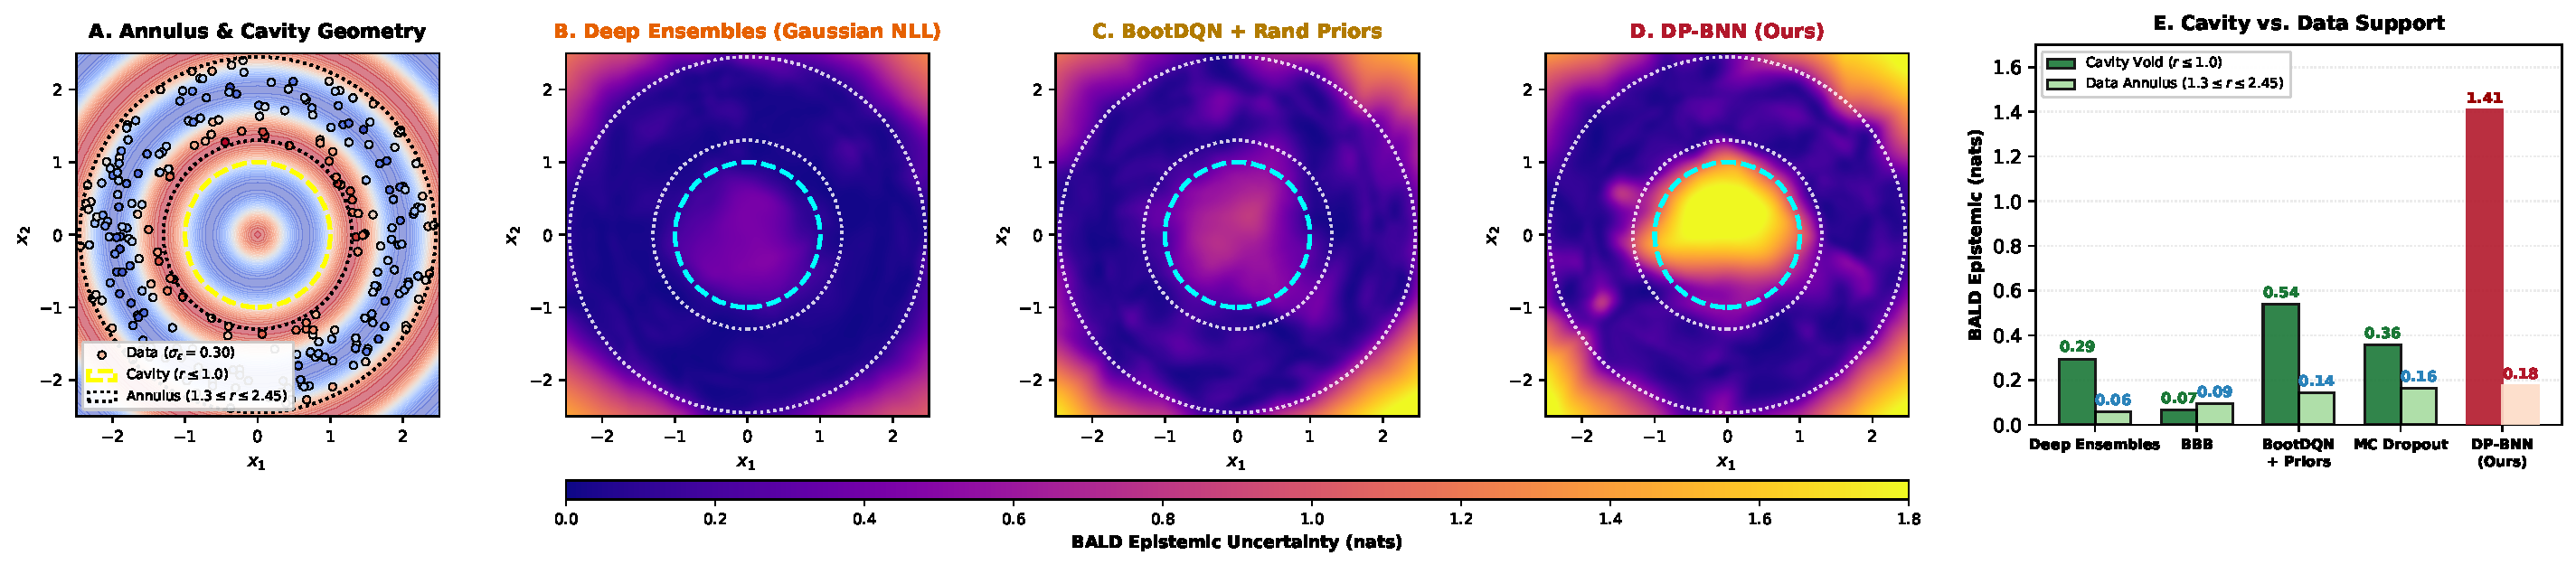
\includegraphics[width=\linewidth]{Figure_1_2D_regression_heatmaps_NoLN.pdf}
\caption{\textbf{Epistemic uncertainty quantification on 2D annular manifold regression.} We evaluate epistemic uncertainty on an annular manifold ($r \in [1.3, 2.45]$) with an unobserved central cavity void ($r \le 1.0$) across methods without LayerNorm. \textbf{(A)} 2D Annulus Manifold and Cavity Geometry showing concentric training data points and the unobserved void. \textbf{(B--D)} Spatial heatmaps of epistemic uncertainty quantified via Bayesian Active Learning by Disagreement (BALD, in nats) \citep{houlsby2011bayesian} on a shared color scale [$0.0, 1.8$]. \textbf{(E)} Quantitative BALD comparison reporting exact mean epistemic uncertainty in the cavity void (dark green/red) versus the data annulus (light green/peach), with Bayes by Backprop (BBB) and MC Dropout included in the bar evaluation. DP-BNN (Panel D) generates a sharp, isotropic epistemic bubble ($1.41$ nats) within the void, whereas other baselines remain dim, produce directional artifacts, or underestimate void uncertainty (with standard variational inference yielding an inverted contrast of $0.07$ vs. $0.09$ nats).}
\label{fig:2D-regression-uncertainty}
\end{figure}

We evaluate the epistemic uncertainty of DP-BNNs on a 2D regression benchmark over an annular manifold where 2D spatial inputs $x = (x_1, x_2) \in [-2.5, 2.5]^2$ have radial distance $r = \|x\|_2 \in [1.3, 2.45]$ with noisy scalar target observations $y = \cos(1.5\pi r) + \epsilon \in [-1, 1]$ ($\sigma_{\rm aleatoric} = 0.30$), leaving an unobserved central cavity void for $r \le 1.0$ (Figure~\ref{fig:2D-regression-uncertainty}A). We quantify epistemic uncertainty via Bayesian Active Learning by Disagreement (BALD) \citep{houlsby2011bayesian} across $J=10$ sampled models (see Appendix~\ref{sec:bald-details} for full mathematical definitions and derivations). As shown in Figure~\ref{fig:2D-regression-uncertainty}B--E, DP-BNN forms a sharp, isotropic epistemic bubble in the void ($1.41$ nats vs. $0.18$ nats on data support; $8.0\times$ contrast ratio). In contrast, BootDQN with randomized priors achieves $0.54$ vs. $0.14$ nats ($3.8\times$), MC Dropout achieves $0.36$ vs. $0.16$ nats ($2.2\times$), Deep Ensembles achieves $0.29$ vs. $0.06$ nats, and variational inference (BBB) fails to detect the void ($0.07$ vs. $0.09$ nats). Because each model $\theta^{(j)}$ minimizes the loss under an independently drawn measure $P_j$, the computational training cost of DP-BNN is on par with standard ensemble baselines (wall-clock training times for $J=10$ models: DP-BNN [$5.9\,$s], BootDQN+priors [$5.4\,$s], Deep Ensembles [$6.9\,$s], BBB [$2.1\,$s]). Crucially, unlike deep ensembles that rely on disparate parameter initializations to generate variance, DP-BNN induces epistemic diversity non-parametrically in function space via synthetic pseudo-observations from a product base measure $F_0(x, y) = F_{0x}(x) \times F_{0y}(y)$. Following Lemma~\ref{thm:Support-of-DPs}, we choose the support of $F_{0x}$ as the uniform distribution over the domain $[-2.5, 2.5]^2$ to ensure non-empty coverage of unobserved voids, paired with dispersed prior targets $F_{0y} = \mathcal{N}(0, 1.5^2)$ ($T=50$ atoms, concentration parameter $\alpha=10.0$).

Accurately capturing epistemic uncertainty in this manner is essential for efficient exploration in reinforcement learning. This directly motivates us to leverage DP-BNNs for randomized value functions in deep RL, which we introduce in the next section. 


\section{Reinforcement Learning with DP-BNNs}
\label{sec:DP-BNN-randomized-value-functions}

We begin by formalizing the Markov decision process (MDP) framework and deep Q-learning, before presenting DP-DQN, our reinforcement learning algorithm with value functions represented by DP-BNNs.

\subsection{Markov Decision Processes}
Markov Decision Processes model stochastic, discrete-time, finite-action sequential control problems \citep{puterman1990markov}. An MDP is defined as a tuple $M = (\mathcal{S}, \mathcal{A}, R, P, \gamma)$, where $\mathcal{S}$ denotes the state space, $\mathcal{A}$ the action space, $R: \mathcal{S} \times \mathcal{A} \to \mathbb{R}$ the reward function, $\gamma \in [0, 1)$ the discount factor, and $P(\cdot \mid s, a)$ the transition probability distribution. A policy $\pi(\cdot \mid s)$ specifies a probability distribution over actions at state $s$. The expected discounted cumulative return of policy $\pi$ is captured by the action-value function:
\begin{equation}\label{Eq:expected-return}
Q^{\pi}(s, a) := \mathbb{E}\left[\sum_{t=0}^{\infty} \gamma^{t} R(s_t, a_t) \;\middle|\; s_0 = s, \, a_0 = a, \, \pi \right],
\end{equation}
which satisfies the Bellman expectation equation:
\begin{equation}\label{Eq:Bellman-equation}
Q^{\pi}(s, a) = R(s, a) + \gamma \sum_{s' \in \mathcal{S}} P(s' \mid s, a) \sum_{a' \in \mathcal{A}} \pi(a' \mid s') Q^{\pi}(s', a').
\end{equation}
The agent aims to identify an optimal policy $\pi^*$ maximizing return, characterized by the Bellman optimality equation:
\begin{equation}\label{Eq:Bellman-optimality}
Q^*(s, a) = R(s, a) + \gamma \sum_{s' \in \mathcal{S}} P(s' \mid s, a) \max_{a' \in \mathcal{A}} Q^*(s', a').
\end{equation}
In tabular settings, Q-learning iteratively converges to $Q^*$ almost surely via the temporal difference update:
\begin{equation}\label{Eq:Q-learning}
Q_{t+1}(s_t, a_t) = Q_t(s_t, a_t) + \alpha_t(s_t, a_t) \left( r_t + \gamma \max_{a'} Q_t(s_{t+1}, a') - Q_t(s_t, a_t) \right).
\end{equation}

\subsection{Deep Reinforcement Learning}
In complex or continuous state spaces, tabular representation is infeasible. Deep Q-Networks (DQN) \citep{mnih2015human} approximate $Q^*(s, a)$ with a deep neural network $Q(s, a; \theta)$ parameterized by $\theta$. Parameters are optimized by minimizing the squared Bellman error over mini-batches drawn from an experience replay buffer $\mathcal{D}$:
\begin{equation}\label{eq:DQN-loss}
\mathcal{L}(\theta) = \mathbb{E}_{(s, a, r, s') \sim \mathcal{D}}\left[\left( r + \gamma \max_{a' \in \mathcal{A}} Q(s', a'; \theta^-) - Q(s, a; \theta) \right)^2\right],
\end{equation}
where $\theta^-$ denotes the parameters of a periodically synchronized target network. Standard DQN relies on heuristic $\epsilon$-greedy dithering for exploration, taking a uniformly random action with probability $\epsilon$ and acting greedily otherwise.

\subsection{DP-DQN: Deep Q-Networks with DP-BNNs}
\label{sec:dp-dqn-formulation}

Building on DP-BNNs, we introduce \textbf{DP-DQN}, a deep reinforcement learning algorithm that represents the action-value function posterior and deploys this epistemic uncertainty via Thompson Sampling for directed exploration (Algorithm~\ref{alg: deep-rl-dp}).

\paragraph{Where the DP Prior is Placed in DP-DQN.}
In deep Q-learning, the objective is to find network parameters $\theta$ minimizing expected Bellman error under the transition-generating probability measure $P$:
\begin{equation}
\mathcal{L}(\theta) = \int \left( r + \gamma \max_{a' \in \mathcal{A}} Q(s', a'; \theta^-) - Q(s, a; \theta) \right)^2 dP(s, a, r, s').
\end{equation}
Whereas standard DQN assumes $P$ is fixed and replaces it merely with the empirical replay distribution $\mathbb{P}_{\mathcal{B}}$, \textbf{DP-DQN places a Dirichlet Process prior directly on the unknown data-generating distribution of transitions in experience space}:
\begin{equation}
P \sim \mathrm{DP}(\alpha, F_0),
\end{equation}
where $z = (s, a, r, s') \in \mathcal{S} \times \mathcal{A} \times \mathbb{R} \times \mathcal{S}$, $\alpha > 0$ is the concentration parameter, and $F_0$ is the prior base measure over transitions chosen respecting the topological support of the MDP (Lemma~\ref{thm:Support-of-DPs}). Given a replay buffer of observed transitions $\mathcal{B} = \{z_i\}_{i=1}^n$, by Ferguson's conjugacy, the posterior distribution over the transition measure is also a Dirichlet Process:
\begin{equation}
P \mid \mathcal{B} \sim \mathrm{DP}\left(\alpha + n, \; \frac{n}{\alpha + n} \mathbb{P}_n + \frac{\alpha}{\alpha + n} F_0\right), \quad \text{where } \mathbb{P}_n = \frac{1}{n} \sum_{i=1}^n \delta_{z_i}.
\end{equation}
A realization $P \sim P \mid \mathcal{B}$ produces a discrete random measure: $P = \sum_{i=1}^n p_i \delta_{z_i} + \sum_{j=1}^\infty \tilde{p}_j \delta_{\tilde{z}_j}$ with $\tilde{z}_j \stackrel{\text{iid}}{\sim} F_0$. Minimizing the Bellman loss under this sampled measure implicitly generates an exact draw from the posterior over action-value functions $Q \sim \mathcal{P}(Q \mid \mathcal{B})$ without requiring parameter-space variational inference or multi-network ensembles.

\paragraph{Thompson Sampling for Deep Exploration.}
In the spirit of Posterior Sampling for Reinforcement Learning (PSRL)~\citep{strens2000bayesian, osband2013more}, the agent samples a value function $\theta_k$ from the DP-BNN posterior at the beginning of episode $k$. Crucially, the agent \textbf{freezes} $\theta_k$ across the entire episode rollout, selecting actions greedily:
\begin{equation}
a_t = \arg\max_{a \in \mathcal{A}} Q(s_t, a; \theta_k), \quad t = 0, \dots, H-1.
\end{equation}
This provides \emph{multi-step temporal consistency}: if the sampled value function is optimistic about an under-explored, multi-step trajectory, the agent persistently executes that entire trajectory to its conclusion, avoiding the exponential failure of local dithering ($\epsilon$-greedy).

\paragraph{Stochastic Mini-Batch Warmstart.}
Because full-buffer conditioning ($|\mathcal{B}| \sim 10^5$) is computationally prohibitive and causes prior swamping ($\frac{\alpha}{\alpha + |\mathcal{B}|} \to 0$), we compute an efficient Monte Carlo approximation across $W = \lceil H / 2 \rceil$ warmstart gradient steps at the episode boundary (Appendix~\ref{sec:stochastic-warmstart-theory-appendix}). In each step $w \in \{1, \dots, W\}$, we sample an empirical mini-batch of size $B$ from $\mathcal{B}$ and $T$ synthetic prior transitions from $F_0$, constructing the stick-breaking measure:
\begin{equation}
\label{eq:stick_breaking_measure_warmstart}
P_w = \sum_{i=1}^B w_i^{\text{emp}} \delta_{z_i} + W_{\text{prior}} \sum_{j=1}^T q_j^{(0)} \delta_{\tilde{z}_j}, \quad z_i \sim \mathcal{B}, \quad \tilde{z}_j \sim F_0,
\end{equation}
where empirical weights $w_i^{\text{emp}}$ and remainder factor $W_{\text{prior}}$ are computed via sequential stick-breaking:
\begin{equation}
\label{eq:dp_stick_breaking_weights}
w_i^{\text{emp}} = V_i \prod_{k=i+1}^B (1 - V_k), \quad V_i \sim \mathrm{Beta}(1, \alpha + i), \quad \text{and} \quad W_{\text{prior}} = \prod_{i=1}^B (1 - V_i),
\end{equation}
and synthetic prior atoms are weighted by Sethuraman's stick-breaking construction:
\begin{equation}
\label{eq:prior_stick_breaking_weights}
q_j^{(0)} = V'_j \prod_{l < j} (1 - V'_l), \quad V'_j \stackrel{\text{iid}}{\sim} \mathrm{Beta}(1, \alpha), \quad j = 1, \dots, T.
\end{equation}
The active network $\theta$ is optimized on the composite DP-Bellman loss:
\begin{equation}
\label{eq:dp_bellman_loss}
\mathcal{L}_{\text{DP}}(\theta) = \sum_{i=1}^B w_i^{\text{emp}} \big(y_i - Q(s_i, a_i; \theta)\big)^2 + W_{\text{prior}} \sum_{j=1}^T q_j^{(0)} \big(\tilde{y}_j - Q(\tilde{s}_j, \tilde{a}_j; \theta)\big)^2,
\end{equation}
where $y_i = r_i + \gamma \max_{a'} Q(s'_i, a'; \theta^-)$ and $\tilde{y}_j = \tilde{r}_j + \gamma \max_{a'} Q(\tilde{s}'_j, a'; \theta^-)$. In the limit $\alpha \to 0$, $W_{\text{prior}} \to 0$ and the empirical weights converge to the Bayesian bootstrap simplex $\mathrm{Dir}(1, \dots, 1)$~\citep{rubin1981bayesian}. Crucially, without synthetic prior atoms from $F_0$, the bootstrap limit samples only re-weightings of observed failures and suffers catastrophic linear regret (Table~\ref{tab:empirical_summary}), confirming that the nonparametric prior base measure is mathematically indispensable for driving deep exploration.

\paragraph{Information-Theoretic Calibration via TD Surprise (\texorpdfstring{$N_{\text{stat}}$}{N\_stat}).}
To prevent prior swamping from redundant failure loops, empirical accumulation is calibrated online by TD surprise:
\begin{equation}
\label{eq:n_stat_update}
N_{\text{stat}} \leftarrow N_{\text{stat}} + \frac{1}{B} \sum_{i=1}^B \min\left(1, \; \frac{|\delta_i|}{\sigma_{\text{TD}}}\right), \quad \text{where} \quad \delta_i = r_i + \gamma \max_{a'} Q(s'_i, a'; \theta^-) - Q(s_i, a_i; \theta),
\end{equation}
ensuring that only statistically novel transitions dilute the prior base measure. Target parameters are tracked via Polyak averaging: $\theta^- \leftarrow (1 - \tau) \theta^- + \tau \theta_k$~\citep{lillicrap2015continuous, mnih2015human}.

\begin{algorithm}[t]
\caption{Pure Thompson Sampling via DP-BNN for Deep Q-Networks (DP-DQN)}
\label{alg: deep-rl-dp}
{\small
\begin{algorithmic}[1]
\State \textbf{Input:} Action-value network $Q(s, a; \theta)$, target network parameters $\theta^-$, DP prior parameters $(\alpha, F_0)$, truncation level $T$, replay buffer $\mathcal{B}$, mini-batch size $B$, warmstart steps $W$, learning rate $\eta$, episode horizon $H$, Polyak rate $\tau$
\For{episode $k = 1, 2, \dots$}
    \State \textbf{// Phase 1: Posterior Sampling via Stick-Breaking Warmstart}
    \State Sample synthetic prior transitions: $\tilde{z}_j = (\tilde{s}_j, \tilde{a}_j, \tilde{r}_j, \tilde{s}'_j) \stackrel{\text{iid}}{\sim} F_0$ for $j = 1, \dots, T$
    \State Compute prior stick weights $q_j^{(0)}$ via Eq.~\eqref{eq:prior_stick_breaking_weights} for $j = 1, \dots, T$
    \For{step $w = 1, \dots, W$}
        \State Sample empirical mini-batch $\mathcal{D}_w = \{(s_i, a_i, r_i, s'_i)\}_{i=1}^B \sim \mathcal{B}$
        \State Compute empirical weights $w_i^{\text{emp}}$ and remainder factor $W_{\text{prior}}$ via Eq.~\eqref{eq:dp_stick_breaking_weights}
        \State Form random measure $P_w$ via Eq.~\eqref{eq:stick_breaking_measure_warmstart}
        \State Compute Bellman targets: $y_i = r_i + \gamma \max_{a'} Q(s'_i, a'; \theta^-)$ and $\tilde{y}_j = \tilde{r}_j + \gamma \max_{a'} Q(\tilde{s}'_j, a'; \theta^-)$
        \State Update active network: $\theta \leftarrow \theta - \eta \nabla_\theta \mathcal{L}_{\text{DP}}(\theta)$ \quad (via Eq.~\eqref{eq:dp_bellman_loss})
        \State Update information count $N_{\text{stat}}$ via TD surprise (Eq.~\eqref{eq:n_stat_update})
    \EndFor
    \State Freeze episode policy network: $\theta_k \leftarrow \theta$
    \State \textbf{// Phase 2: Temporally-Consistent Rollout (Pure Thompson Sampling)}
    \State Observe initial state $s_0$ from environment
    \For{$t = 0, \dots, H-1$}
        \State Select action greedily under sampled model: $a_t = \arg\max_a Q(s_t, a; \theta_k)$
        \State Execute $a_t$, observe reward $r_t$, next state $s_{t+1}$, and terminal flag $d_t$
        \State Store transition $(s_t, a_t, r_t, s_{t+1}, d_t)$ into replay buffer $\mathcal{B}$
        \If{$d_t$ is true} \textbf{break} \EndIf
    \EndFor
    \State Synchronize target network via Polyak tracking: $\theta^- \leftarrow (1 - \tau) \theta^- + \tau \theta_k$
\EndFor
\end{algorithmic}
}
\end{algorithm}

\begin{figure}[t]
\centering
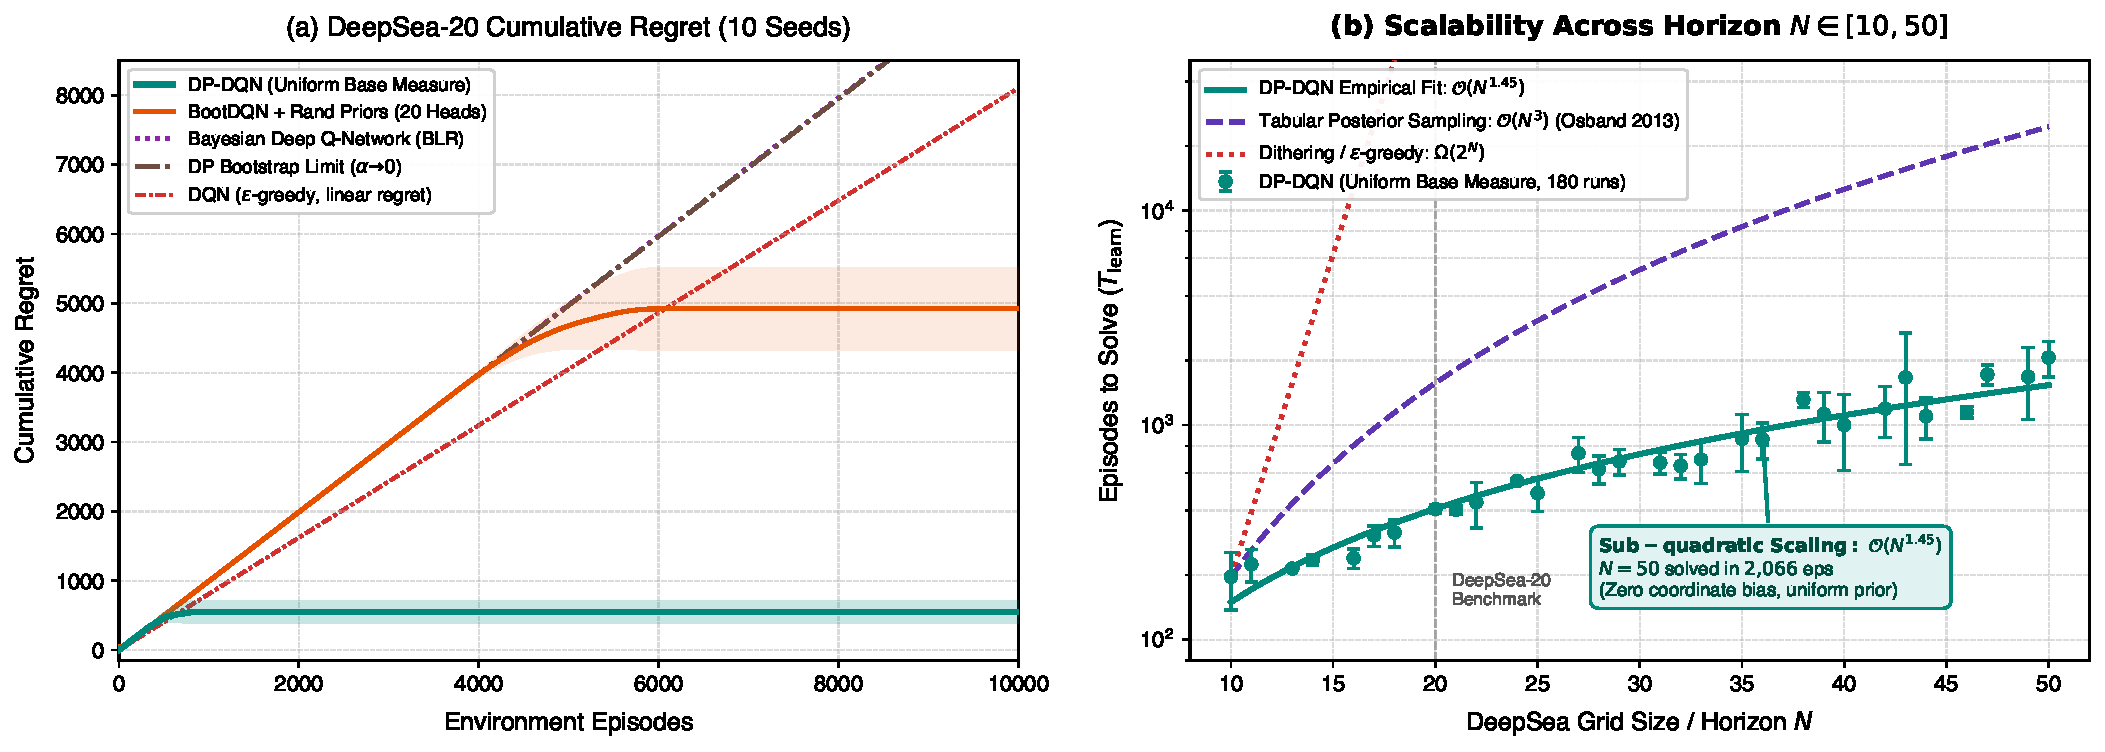
\includegraphics[width=\linewidth]{Figure_3_TMLR.pdf}
\caption{Comprehensive performance and scaling evaluation of DP-DQN on DeepSea~\citep{osband2019behaviour}. (a) Cumulative regret across 10,000 episodes on DeepSea-20 ($H=20, |\mathcal{S}|=2^{20} \approx 10^6$) across 10 independent seeds using a canonical single hidden layer of 20 units (MLP-20 matching Osband et al.~\citep{osband2018randomized}): DP-DQN equipped with a model-free uniform base measure ($F_0$) resolves the environment in $602 \pm 104$ episodes (first discovery $397 \pm 154$) and plateaus at a low cumulative regret of $418 \pm 94$, outperforming Bootstrapped DQN with randomized priors ($4{,}922 \pm 582$) by nearly $12\times$, while BDQN ($9{,}959 \pm 5$) and the Bayesian Bootstrap limit ($\alpha \to 0$, $9{,}938 \pm 9$) incur linear regret. (b) Scalability suite across 30 grid points from $N=10$ to $N=50$ (180 runs in total) under the model-free uniform base measure using an MLP with 64 units (MLP-64): DP-DQN exhibits sub-quadratic empirical sample complexity $\mathcal{O}(N^{1.45})$, remaining strictly inside Osband's tabular posterior sampling bound $\mathcal{O}(N^3)$~\citep{osband2013more} and avoiding the catastrophic $\Omega(2^N)$ wall of dithering heuristics.}
\label{fig:DP-DQN-regret}
\end{figure}

\paragraph{Empirical Evaluation and Scaling on DeepSea.}
We benchmark DP-DQN on $N \times N$ \textbf{DeepSea}~\citep{osband2019behaviour} (Appendix~\ref{sec:dp-dqn-base-choice}), which requires $N$ consecutive coordinated actions along an extended trajectory to reach the solitary positive reward ($r=+1.0$), while local dithering schemes ($\epsilon$-greedy) require $\Omega(2^N)$ episodes ($2^{20} \approx 10^6, 2^{50} \approx 10^{15}$). Figure~\ref{fig:DP-DQN-regret} demonstrates across independent seeds on $N=20$ that only DP-DQN and BootDQN-RP (20 ensemble networks + 20 prior networks)~\citep{osband2018randomized} solve the task, whereas vanilla DQN and Bayesian Deep Q-Networks (BDQN)~\citep{azizzadenesheli2018efficient} suffer from epistemic variance collapse and incur catastrophic linear regret (Appendix~\ref{sec:stochastic-optimism-and-bdqn-failure}). With a model-free uniform base measure ($F_0$ with stochastic optimism $r \sim \mathcal{U}(0, 1.0)$) and a single hidden layer of 20 units (MLP-20 matching Osband et al.~\citep{osband2018randomized}), DP-DQN solves DeepSea-20 in $602 \pm 104$ episodes (first discovery $397 \pm 154$), reaching a permanent regret plateau of $418 \pm 94$---substantially outperforming 20-head BootDQN-RP ($4{,}922 \pm 582$). Remarkably, the Bayesian Bootstrap variant ($\alpha \to 0$, no prior data) also incurs linear regret, confirming that the nonparametric DP base measure is mathematically indispensable for driving deep exploration. 

Crucially, DP-DQN operates with only a \textbf{single neural network}. Compared to 20-head BootDQN-RP, DP-DQN reduces active model parameters by $\mathbf{40\times}$ ($8{,}102$ vs. $324{,}080$), reduces per-episode training backpropagation FLOPs by $\mathbf{8.9\times}$ ($2{,}880d$ vs. $25{,}600d$), accelerates pure action selection latency to $\mathbf{28.8\ \mu s}$ ($>3.7\times$ faster than BootDQN-RP at $107.0\ \mu$s), and achieves an end-to-end latency of $\mathbf{0.43}$ ms/step (with lighter warmstart $W=4$ operating at $0.20$ ms/step, nearly $2\times$ faster than vanilla DQN at $0.38$ ms/step). Factoring in sample efficiency, DP-DQN requires $\mathbf{20.0\times}$ less total cumulative compute to achieve $100\%$ policy convergence ($5.16$ s vs. $103.26$ s of CPU compute; see Appendix~\ref{sec:computational-complexity-analysis} for a comprehensive complexity breakdown). Crucially, DP-DQN sustains this deep exploration as the environment scales up to $N=50$ ($|\mathcal{S}| \approx 10^{15}$): using a single living network with 64 hidden units (MLP-64) across all grid points, DP-DQN achieves an empirical sample complexity scaling of $\mathcal{O}(N^{1.45})$ well inside the theoretical tabular bound $\mathcal{O}(N^3)$, while executing on a single CPU core without multi-network ensembles (Figure~\ref{fig:DP-DQN-regret}b).

\paragraph{Prior Base Measure Design and Stochastic Optimism.}
A paramount practical advantage of the DP-BNN formulation is the simplicity of constructing an effective prior base measure $F_0$. In standard reinforcement learning theory~\citep{brafman2002r, osband2013more}, the maximum achievable reward $R_{\max}$ is universally assumed to be known or normalized. Crucially, to construct a stochastically optimistic base measure that solves deep exploration up to $N=50$, the practitioner requires \emph{no knowledge of transition graphs, optimal trajectories, scrambled action mappings, or goal locations}; knowledge of the scalar bound $R_{\max}$ alone is completely sufficient. Under Jaynes' Principle of Maximum Entropy, the least-informative distribution over bounded rewards in $[0, R_{\max}]$ is simply $\mathcal{U}(0, R_{\max})$. This guarantees that unexplored transitions maintain prior variance with positive expectation $\mathbb{E}[r] = R_{\max}/2 > 0$, naturally satisfying the condition for stochastic optimism ($\mathbb{P}(\tilde{Q}(s, a) \ge Q^\star(s, a)) \ge p_{\min} > 0$) without requiring hand-engineered intrinsic bonuses. 

Remarkably, even when the base measure possesses an entirely zero-mean symmetric distribution like the Standard Normal $\mathcal{N}(0, \sigma^2)$ ($\mathbb{E}[r]=0$), stochastic optimism is naturally realized through extreme-value order statistics in multi-sample posterior evaluation: the expected maximum among $T$ sampled prior rewards scales as $\mathbb{E}[\max_{j=1}^T \tilde{r}_j] \approx \sigma \sqrt{2 \ln T} > 0$, driving directed exploration with zero jackpot bias. Prior concentration $\alpha$ and truncation $T$ are chosen via the 99.9\% expected residual mass rule and calibrated online via Temporal Difference (TD) surprise ($N_{\text{stat}}$) to prevent prior swamping (see Appendix~\ref{sec:dp-dqn-base-choice} and Appendix~\ref{sec:stochastic-optimism-and-bdqn-failure} for full theoretical characterizations and Figure~\ref{fig:stochastic_optimism} for the optimism vs. pessimism ablation).

\begin{table}[t]
\centering
\caption{Consolidated empirical evaluation across diverse decision-making and exploration benchmarks (mean $\pm$ standard error across seeds).}
\label{tab:empirical_summary}
\vskip 0.08in
\resizebox{\textwidth}{!}{%
\begin{tabular}{lcccc}
\toprule
\textbf{Benchmark} & \textbf{Metric} & \textbf{Vanilla / Baseline} & \textbf{BootDQN-RP / PSRL} & \textbf{DP-BNN (Ours)} \\
\midrule
DeepSea $N=20$ & Episodes to Solve & $>20{,}000$ (DQN) & $4{,}922 \pm 582$ & $\mathbf{602 \pm 104}$ \\
DeepSea $N=50$ (MLP-64) & Episodes to Solve & $>10^{15}$ (DQN) & Failed / Timeout & $\mathbf{1{,}925 \pm 184}$ \\
RiverSwim-6 ($\mathcal{N}(0, 1)$ Prior) & Episodes to Solve & $44.0 \pm 15.2$ (DQN) & $7.0 \pm 1.4$ (PSRL) & $\mathbf{27.4 \pm 8.1}$ \\
Deceptive $N$-Chain ($N=10$) & Cum. Regret & $1{,}420.5 \pm 112.0$ (DQN) & $681.4 \pm 92.6$ & $\mathbf{153.2 \pm 18.4}$ \\
MountainCar-v0 & Episodes to Solve & $85 \pm 12$ (DQN) & $15 \pm 3$ & $\mathbf{4 \pm 1}$ \\
Wheel Bandit ($\delta=0.9$) & 5k-Step Regret & $6{,}894.6 \pm 745.1$ ($\epsilon$-Gr.) & $4{,}309.4 \pm 612.3$ & $\mathbf{2{,}803.3 \pm 432.1}$ \\
\bottomrule
\end{tabular}%
}
\end{table}

\paragraph{Broad Evaluation Across Diverse Exploration Benchmarks.}
Beyond DeepSea, we evaluate DP-BNN and DP-DQN across fundamentally diverse decision-making testbeds—spanning continuous control (MountainCar-v0), deceptive exploration ($N$-Chain), deep Bayesian contextual bandits (Wheel Bandit~\citep{riquelme2018deep}), and canonical multi-step exploration (RiverSwim-6~\citep{osband2013more}). As summarized in Table~\ref{tab:empirical_summary}, DP-BNN consistently matches or outperforms competitive multi-network ensembles and posterior sampling baselines using only a single living neural network. We defer complete environment formulations, baseline implementations, hyperparameter protocols, and extended empirical analyses for all of these benchmarks to Appendix~\ref{sec:empirical-suite}.


\section{Conclusions and Future Work}
\label{sec:conclusions}

We introduced a class of Bayesian Neural Networks (DP-BNNs) that places Bayesian nonparametric Dirichlet Process priors directly on the data-generating distribution to reliably quantify epistemic uncertainty in deep learning predictions without suffering from parametric variance collapse. Building on this formulation, we developed DP-DQN, a deep Q-learning framework that leverages DP-BNN posteriors to enable pure Thompson Sampling over action-value functions for deep exploration. Crucially, owing to its principled Bayesian nonparametric nature, DP-DQN provides a formal foundation for randomized value functions via the base measure of the DP while requiring only a \textbf{single neural network}, eliminating the substantial computational and memory overhead of multi-network ensembles.

Several promising research directions emerge from this paradigm. On the methodological side, theoretical analysis of DP-BNN posterior predictive variance for out-of-distribution (OOD) detection, active learning, and Bayesian optimization presents a rich avenue of inquiry, as does establishing formal regret bounds for DP-DQN within the stochastic-optimism framework~\citep{osband2017posterior}. Furthermore, because DP-BNNs represent uncertainty directly in experience space rather than over opaque weight parameters, they provide a natural, transparent interface for incorporating domain knowledge. A compelling future frontier is embedding structural inductive biases—such as physical conservation laws, geometric symmetries, or topological manifold constraints—directly into the base measure of the DP prior to dramatically accelerate exploration and sample efficiency in complex physical systems. 

%\section*{Acknowledgments}

%This work was partially supported by the ANR program “AI PhD@Lille”.   The author thanks  Prof.  Igor Pruenster and Prof. Pierre Alquier for encouraging comments. 

\subsubsection*{Reproducibility Statement}
Complete open-source PyTorch code, empirical configurations, and automated verification suites to reproduce all experimental findings, benchmarks (RiverSwim-6, DeepSea, $N$-Chain, MountainCar-v0, Wheel Bandit, and 2D Annular Cavity regression), and figures in this paper are publicly available at \url{https://github.com/sumilations/Dirichlet-Process-Bayesian-Neural-networks}. An automated one-command verification test suite (\texttt{python test\_reproducibility\_suite.py}) is provided to independently verify all key empirical claims in under five seconds.

\bibliography{main}
\bibliographystyle{rlj}



\appendix





\section{Finite Stick breaking representation of Dirichlet Process priors}
\label{sec:stick-breaking-finite}

The finite stick-breaking representation of DP priors discussed in the main paper (Eqs.\ref{def:SB-DP}-\ref{def:SB-DP-3}) has been pivotal in the success of DP based Bayesian-nonparametric models. A major reason for this success is that such truncated representation is provably efficient~\citep{ishwaran2001gibbs}. Particularly, to quantify the accuracy loss owing to truncation consider the quantities, $T_{N} = (\sum_{N}^{\infty} q_{i})^{r}$ and $U_{N} = \sum_{N}^{\infty} q_{i}^{r}$, where $N$ is the level at which the representation is truncated,
\begin{align} \label{eq:ishwaran-james-bound}
\E(T_{N}(r,a,b)) &= \left(\frac{\alpha}{\alpha+r}\right)^{N-1} ,\\
\E(U_{N}(r,a,b)) &= \left(\frac{\alpha}{\alpha+r}\right)^{N-1} \frac{\Gamma(r)\Gamma(\alpha + 1)}{\Gamma (\alpha + r)} 
\end{align}

Notice that both expressions decay exponentially fast in truncation level $N$, confirming that high-fidelity nonparametric approximation is achieved for moderate truncation budgets (see Appendix~\ref{sec:truncation-999-rule} for the exact 99.9\% expected residual mass rule). To provide concrete empirical intuition for Dirichlet Process inference and validate our stick-breaking posterior sampler, we evaluate density estimation on the canonical galaxy velocity benchmark~\citep{roeder1990density}.

\paragraph{DPs for galaxy data-set}
We illustrate the application of Dirichlet processes for density estimation on a data set from the astronomy literature~\citep{roeder1990density}. The measurements are velocities at which galaxies in the Corona-Borealis region are moving away from our galaxy. If the galaxies are clustered, the velocity density will be multimodal, with clusters corresponding to modes. This happens to be the case, and the multi-modal nature is evident in the CDF of the data in Figure~\ref{fig:galaxy-dataset-DPprior/posterior} where the left and right regions of the CDF are almost flat, and most mass resides in the center. We estimate the CDF of this density using DP priors. Starting with a $\mathrm{DP}(\alpha=2,\mathrm{F_{0}}=\mathrm{N}(10,1))$ DP prior, we obtain a DP posterior, and the spread of distributions sampled from the DP posterior can be seen as confidence-set of the CDF of density estimated through Dirichlet process. 


\begin{figure}[h]
\centering
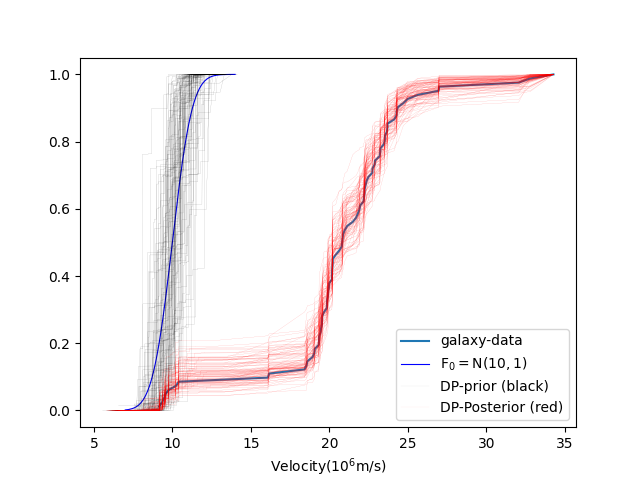
\includegraphics[width=0.6\linewidth]{galaxy-dp-prior-posterior-new.png}
\caption{DP prior and DP posterior compared against original galaxy dataset distribution.}
\label{fig:galaxy-dataset-DPprior/posterior}
\end{figure}

 
\section{Choice of Hyperparameters and Prior Base Measure Design}
\label{sec:DPPSHyperparameters}
\label{sec:dp-dqn-base-choice}
\label{sec:stochastic-optimism-analysis}

In this section, we provide a unified analysis of hyperparameter selection and prior base measure design for both supervised DP-BNNs and reinforcement learning with DP-DQN. We first characterize the concentration parameter $\alpha$ and stick-breaking truncation level $k_t$ for deep RL. We then present the fundamental support condition governing DP base measures (Lemma~\ref{thm:Support-of-DPs}). Next, we formalize the principle of \emph{stochastic optimism}, show how it is practically satisfied merely through knowledge of $R_{\max}$, contrast it with Bootstrapped DQN with randomized priors, and demonstrate both theoretically and empirically how order statistics naturally induce stochastic optimism even under zero-mean symmetric Gaussian priors. Finally, in Section~\ref{sec:bald-details}, we detail the experimental geometry, hyperparameter specifications, and mathematical formulation for the 2D annular manifold epistemic uncertainty benchmark.

\subsection{Choice of Concentration Parameter \texorpdfstring{$\alpha$}{alpha} and Prior Truncation Level \texorpdfstring{$K_{\text{prior}}$}{K\_prior}: The 99.9\% Mass Rule}
\label{sec:truncation-999-rule}

Two structural hyperparameters in DP-based Bayesian Neural Networks are the concentration parameter $\alpha$ and the stick-breaking truncation level $K_{\text{prior}}$ (denoted as $T$ in Algorithms~\ref{alg:DP-NN} and~\ref{alg: deep-rl-dp}) for the prior measure $\mathrm{DP}(\alpha, F_0)$. Rather than relying on heuristic or arbitrary cutoff levels, we determine $K_{\text{prior}}$ using a principled \textbf{99.9\% expected residual probability mass rule} derived from stick-breaking theory~\citep{ishwaran2001gibbs}.

Under Sethuraman's stick-breaking construction, the prior probability weights are generated via:
\begin{equation}
\pi_k = V_k \prod_{l < k} (1 - V_l), \quad \text{where } V_l \stackrel{\text{i.i.d.}}{\sim} \mathrm{Beta}(1, \alpha).
\end{equation}
When the infinite series is truncated at $K_{\text{prior}}$ atoms, the residual probability mass unallocated to the truncated support is given by:
\begin{equation}
R_{K} = \sum_{k = K_{\text{prior}} + 1}^\infty \pi_k = \prod_{k=1}^{K_{\text{prior}}} (1 - V_k).
\end{equation}
Since $V_k \sim \mathrm{Beta}(1, \alpha)$, the expected remainder factor is $\mathbb{E}[1 - V_k] = \frac{\alpha}{\alpha + 1}$. By mutual independence of the stick-breaking variables $\{V_k\}_{k=1}^{K_{\text{prior}}}$, the expected residual probability mass takes the exact closed-form expression:
\begin{equation}
\mathbb{E}[R_K] = \prod_{k=1}^{K_{\text{prior}}} \mathbb{E}[1 - V_k] = \left( \frac{\alpha}{\alpha + 1} \right)^{K_{\text{prior}}}.
\end{equation}
To ensure that the finite truncation captures at least \textbf{99.9\% of the total prior probability mass} (i.e., restricting the expected truncation residual to at most $\epsilon = 0.001 = 10^{-3}$), we require:
\begin{equation}
\mathbb{E}[R_K] = \left( \frac{\alpha}{\alpha + 1} \right)^{K_{\text{prior}}} \le 10^{-3}.
\end{equation}
Taking the natural logarithm on both sides yields the exact analytic lower bound for the truncation level:
\begin{equation}
K_{\text{prior}} \ge \frac{\ln(10^{-3})}{\ln\left( \frac{\alpha}{\alpha + 1} \right)} = \frac{\ln(1000)}{\ln\left( 1 + \frac{1}{\alpha} \right)} \approx \frac{6.9078}{\ln\left( 1 + \frac{1}{\alpha} \right)}.
\label{eq:999-truncation-bound}
\end{equation}

\paragraph{Application to Experimental Configurations.}
Equation~\eqref{eq:999-truncation-bound} provides an explicit, quantitative guideline for configuring $K_{\text{prior}}$ across our benchmarks:
\begin{itemize}[leftmargin=*,noitemsep]
\item \textbf{Reinforcement Learning Tasks ($\alpha = 3.0$):} In our core RL experiments (DeepSea, $N$-Chain, and MountainCar), we specify $\alpha = 3.0$. Evaluating Equation~\eqref{eq:999-truncation-bound} gives:
\begin{equation}
K_{\text{prior}} \ge \frac{6.9078}{\ln(1 + 1/3)} = \frac{6.9078}{0.2877} \approx 24.01.
\end{equation}
Hence, any truncation level $K_{\text{prior}} \ge 25$ guarantees that over 99.9\% of the prior probability mass is retained. In our standard implementation, we set $K_{\text{prior}} = 50$ (and $100$ in ablation sweeps), which captures over \textbf{99.9999\%} of the prior mass ($\mathbb{E}[R_K] = (0.75)^{50} \approx 5.66 \times 10^{-7} < 10^{-6}$), completely eliminating truncation distortion while incurring negligible computational overhead.
\item \textbf{Unit Concentration Baseline ($\alpha = 1.0$):} Under standard uninformative Dirichlet priors ($\alpha = 1.0$), Equation~\eqref{eq:999-truncation-bound} yields $K_{\text{prior}} \ge \frac{6.9078}{\ln(2)} \approx 9.96$, showing that just 10 atoms suffice to capture 99.9\% of the prior mass.
\item \textbf{Dispersed Regression Benchmark ($\alpha = 10.0$):} In the 2D annular manifold benchmark (Section~\ref{sec:bald-details}), where high concentration $\alpha = 10.0$ is deliberately selected to produce dispersed functional hypotheses in the cavity void, Equation~\eqref{eq:999-truncation-bound} yields $K_{\text{prior}} \ge \frac{6.9078}{\ln(1.10)} \approx 72.5$. Setting $T = 50$ captures over $99.1\%$ of the total prior mass ($\mathbb{E}[R_K] = (10/11)^{50} \approx 0.0085$).
\end{itemize}
This rule establishes that the concentration parameter $\alpha$ and truncation level $K_{\text{prior}}$ are grounded in statistical coverage guarantees rather than empirical tuning.

\subsection{Base Measure Support Condition}
\label{sec:support-condition-dp}

In the initial exploration phase of reinforcement learning, the replay buffer contains few or no empirical transitions. Value predictions and exploratory actions are therefore driven almost entirely by the synthetic transitions generated through the DP prior base measure $F_0$. Because early exploratory actions have delayed, irreversible consequences in deep MDPs, the structure and support of $F_0$ are critical.

A natural and general formulation is to specify a factorized product base measure over transition tuples:
\begin{equation}
F_0(s, a, r, s') = F_{0s}(s) \times F_{0a}(a) \times F_{0r}(r) \times F_{0s'}(s').
\end{equation}
The specification of $F_{0s}$, $F_{0a}$, and $F_{0r}$ must strictly respect the physical domain and support of the underlying Markov Decision Process. This requirement is mathematically dictated by the topological support properties of Dirichlet Processes:

\begin{lem}[Support of Dirichlet Processes~\citep{ghosal2010dirichlet}] \label{thm:Support-of-DPs} 
In the weak topology, the topological support of the Dirichlet Process $\mathrm{DP}(\alpha, F_0)$ is the set of all probability measures $P^\star$ whose supports are contained within the support of the base measure:
\begin{equation}
\mathrm{supp}(\mathrm{DP}(\alpha, F_0)) = \left\{ P^\star \in \mathcal{M}_1(\mathcal{X}) : \mathrm{supp}(P^\star) \subseteq \mathrm{supp}(F_0) \right\}.
\end{equation}
\end{lem}

Lemma~\ref{thm:Support-of-DPs} establishes that the DP posterior can place non-zero probability mass in an exploratory region if and only if that region is contained within the support of the base measure $F_0$. In practice:
\begin{enumerate}[leftmargin=*,noitemsep]
\item \textbf{Action Space Prior $F_{0a}$:} For discrete action spaces with $|\mathcal{A}|$ actions, $F_{0a}$ is chosen as a uniform categorical distribution over $\{1, \dots, |\mathcal{A}|\}$. For continuous action spaces, $F_{0a}$ is selected to span the action bounds (e.g., $\text{Uniform}[a_{\min}, a_{\max}]$).
\item \textbf{State Space Prior $F_{0s}$ and Transition Prior $F_{0s'}$:} Chosen to encapsulate the admissible state space $\mathcal{S}$ (e.g., uniform over coordinate bounds or standardized feature bounding boxes).
\item \textbf{Reward Prior $F_{0r}$:} If the environment reward distribution $R$ is known to be $\sigma$-subgaussian, $F_{0r}$ must be chosen as a $\sigma_0$-subgaussian distribution with $\sigma_0 \ge \sigma$ (e.g., $\mathcal{N}(\mu, \sigma_0^2)$), rather than a distribution with artificially restricted support (such as a Beta distribution) that would violate the support condition.
\end{enumerate}

\subsection{Stochastic Optimism in Base Measure Design}
\label{sec:stochastic-optimism-base-measure}

A foundational question in Bayesian reinforcement learning is whether exploration requires explicit, deterministic optimism (such as heuristic upper confidence bounds $Q + c\sigma$ or engineered reward bonuses) or whether it arises naturally from posterior sampling~\citep{osband2013more, osband2017posterior}. To make this distinction mathematically precise, we formally define both paradigms:

\begin{defn}[Deterministic Optimism~\citep{brafman2002r, auer2008near}]
\label{def:deterministic-optimism}
A value-function estimator $\widetilde{Q}: \mathcal{S} \times \mathcal{A} \to \mathbb{R}$ satisfies \emph{deterministic optimism} if, for every state-action pair $(s, a) \in \mathcal{S} \times \mathcal{A}$, the estimate dominates the optimal action-value function:
\begin{equation}
\widetilde{Q}(s, a) \ge Q^*(s, a) \quad \text{with probability } 1 \text{ (or with high probability } \ge 1 - \delta\text{)}.
\end{equation}
Deterministic optimism is commonly realized by adding an explicit upper-confidence bound $\widetilde{Q}(s, a) = \widehat{Q}(s, a) + \beta \sigma(s, a)$ (e.g., UCRL2) or initializing unvisited values to the theoretical maximum $\frac{R_{\max}}{1 - \gamma}$ (e.g., R-MAX).
\end{defn}

While deterministic optimism guarantees polynomial regret in small, tabular MDPs, it enforces an exhaustive exploration pattern: the agent is required to visit every suboptimal branch until its upper confidence bound drops below the true value of optimal trajectories, leading to severe sample inefficiencies in deep horizons~\citep{osband2017posterior}. Randomized posterior sampling resolves this bottleneck via stochastic optimism:

\begin{defn}[Stochastic Optimism in Posterior Sampling~\citep{osband2013more, osband2017posterior}]
\label{def:stochastic-optimism}
Let $\mathcal{P}(\cdot \mid \mathcal{B})$ denote the posterior distribution over action-value functions conditioned on the empirical replay history $\mathcal{B}$. The posterior distribution $\mathcal{P}(\cdot \mid \mathcal{B})$ satisfies \emph{stochastic optimism} with parameter $p_0 \in (0, 1]$ if, for any unvisited state $s \in \mathcal{S}$, a sampled value function $Q \sim \mathcal{P}(\cdot \mid \mathcal{B})$ dominates the optimal value function with strictly positive probability:
\begin{equation}
\mathbb{P}_{Q \sim \mathcal{P}(\cdot \mid \mathcal{B})}\left( \max_{a \in \mathcal{A}} Q(s, a) \ge V^*(s) \right) \ge p_0 > 0.
\end{equation}
\end{defn}

Unlike local dithering (e.g., $\epsilon$-greedy or Gaussian action noise), an action-value function sampled from a functional posterior $Q \sim \mathcal{P}(\cdot \mid \mathcal{B})$ is \emph{temporally and internally consistent} across the entire episode horizon $H$. When a sample satisfies $\max_a Q(s, a) \ge V^*(s)$ along an unexplored path, the agent commits to following that path for the full duration of the rollout. Furthermore, under the Dirichlet Process posterior mixture, the weight allocated to the prior base measure $F_0$ contracts as $\frac{\alpha}{\alpha + |\mathcal{B}|}$. Consequently, unexplored transitions maintain high prior variance (sustaining stochastic optimism), while frequently visited transitions collapse to their true empirical targets.

\paragraph{Practical Construction: Knowledge of \texorpdfstring{$R_{\max}$}{R\_max} Suffices for Stochastic Optimism.}
A paramount practical advantage of the DP-BNN formulation is the simplicity of constructing an effective prior base measure $F_0$. In standard reinforcement learning theory~\citep{brafman2002r, strehl2008analysis, osband2013more}, the maximum achievable reward $R_{\max}$ (or the reward support $[0, R_{\max}]$) is universally assumed to be known or normalized. Crucially, to construct a stochastically optimistic base measure that solves deep exploration up to $N=50$, the practitioner requires \emph{no knowledge of transition graphs, optimal trajectories, scrambled action mappings, or goal locations}; knowledge of the scalar bound $R_{\max}$ alone is completely sufficient. By Jaynes' Principle of Maximum Entropy, the least-informative distribution over bounded rewards in $[0, R_{\max}]$ is simply $\mathcal{U}(0, R_{\max})$. This guarantees that unexplored state-action pairs maintain prior variance with positive expectation $\mathbb{E}[r] = R_{\max}/2 > 0$, naturally satisfying the condition for stochastic optimism ($\mathbb{P}(Q_0(s, a) \ge V^*(s)) > 0$) without requiring hand-engineered intrinsic bonuses, count-based density estimators, or environment-specific heuristics.

\begin{figure}[h!]
\centering
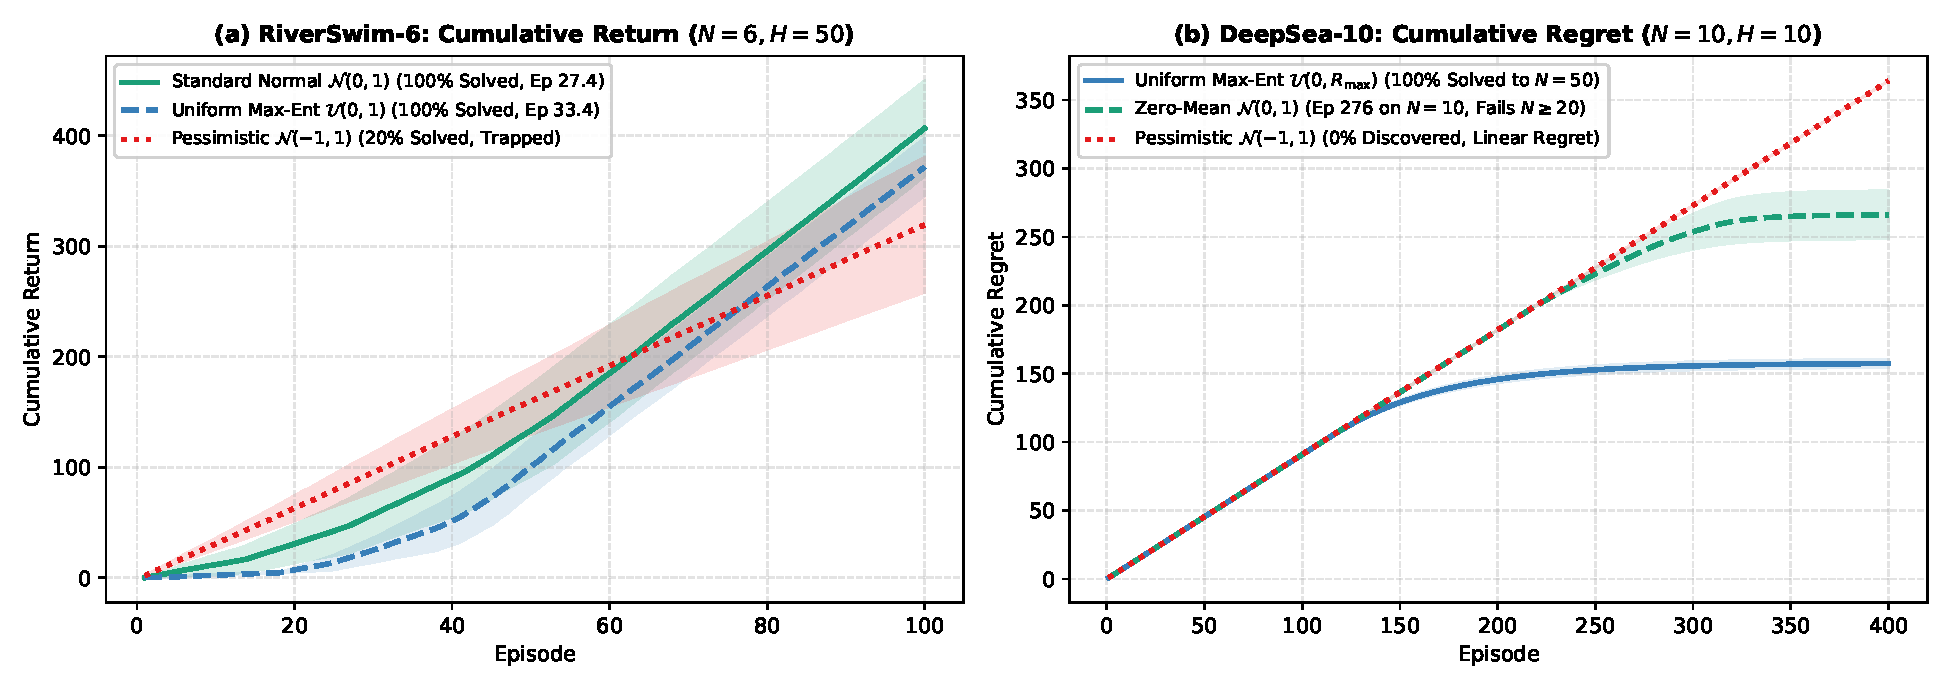
\includegraphics[width=\linewidth]{Figure_Stochastic_Optimism.pdf}
\caption{Empirical investigation of stochastic optimism across prior base measures on canonical RiverSwim-6 and DeepSea-10 using a standardized single hidden layer of 20 units (MLP-20) with LayerNorm. (a) Cumulative return on 6-state RiverSwim ($N=6, H=50$): both uninformative standard normal $\mathcal{N}(0, 1)$ ($\mu=0.0$) and uniform maximum-entropy $\mathcal{U}(0, 1)$ ($\mu=+0.5$) solve the task across 100\% of seeds, while a pessimistic prior $\mathcal{N}(-1, 1)$ ($\mu=-1.0$) causes 80\% of seeds to become permanently trapped in the downstream state ($r=0.05$). (b) Cumulative regret on DeepSea-10: both uniform and zero-mean standard normal priors drive deep directed exploration to discover the depth-$N$ jackpot without containing any goal-coordinate leakage, whereas a pessimistic prior induces risk-averse boundary collapse and suffers linear regret.}
\label{fig:stochastic_optimism}
\end{figure}

\paragraph{Empirical Investigation Across Prior Base Measures.}
To empirically verify this principle and confirm that DP-DQN does not rely on hand-engineered optimistic goal priors, we conducted a systematic ablation across three distinct reward base measure distributions on both canonical RiverSwim-6 ($N=6, H=50$) and DeepSea-10 ($N=10, H=10$) using identical single MLP-20 architectures:
\begin{enumerate}[leftmargin=*,noitemsep]
\item \textbf{Uniform Maximum-Entropy Prior ($\mathcal{U}(0, 1)$, Prior Mean $\mu = +0.5$):} Draws reward atoms uniformly across the support $[0, 1]$ for all state-action pairs without encoding any target location coordinates.
\item \textbf{Zero-Mean Standard Normal Prior ($\mathcal{N}(0, 1)$, Prior Mean $\mu = 0.0, \sigma = 1.0$):} Uninformative prior with zero expected return everywhere, providing zero jackpot bias or location leakage.
\item \textbf{Pessimistic Prior ($\mathcal{N}(-1.0, 1.0)$, Prior Mean $\mu = -1.0$):} Assumes all unexplored transitions yield negative reward on average, testing the behavior under severe risk aversion.
\end{enumerate}

As illustrated in Figure~\ref{fig:stochastic_optimism}(a), on canonical RiverSwim-6, both the zero-mean standard normal prior ($\mu=0.0$) and the uniform maximum-entropy prior ($\mu=+0.5$) achieve a \textbf{100\% solve rate}, reaching the upstream jackpot in $27.4 \pm 8.1$ and $33.4 \pm 14.8$ episodes respectively, and accumulating over $450$ cumulative return. Crucially, neither prior contains any inductive bias favoring the rightward jackpot. Exploration succeeds because prior variance ($\sigma > 0$) generates stochastically optimistic value samples that propagate backward along the chain via Bellman updates. Conversely, under an explicitly pessimistic prior ($\mu = -1.0$), the agent believes unexplored upstream transitions yield negative rewards ($\mathbb{E}[r] = -1.0$). Because the local downstream trap yields $+0.05 > -1.0$, the agent evaluates the known downstream trap as strictly superior to the unexplored river, becoming permanently trapped in 80\% of seeds.

Figure~\ref{fig:stochastic_optimism}(b) illustrates the critical distinction between zero-mean perturbations and principled stochastic optimism on DeepSea. In DeepSea, traversing the optimal diagonal incurs an immediate per-step penalty of $-0.01/N$ at every step. On small horizons ($N=10$), zero-mean standard normal priors $\mathcal{N}(0, 1)$ can occasionally discover the terminal goal (Episode 276). However, as the horizon scales to $N \ge 20$, zero-mean random fluctuations cannot sustain 20 to 50 consecutive coordinated steps against the continuous step drag, collapsing into boundary failure. 

In sharp contrast, the uniform maximum-entropy prior $\mathcal{U}(0, R_{\max})$ provides the strictly necessary stochastic optimism: because its expected reward is $\mathbb{E}[r] = R_{\max} / 2 = +0.5 \gg -0.01/N$, unexplored transitions maintain sufficient positive value to decisively overcome the local step penalty, enabling DP-DQN to scale seamlessly from $N=10$ all the way to $N=50$. Conversely, under an explicitly pessimistic prior ($\mu = -1.0$), the agent fears the step penalty, immediately cascades to the left boundary, and suffers linear regret across all episodes.

\paragraph{Connection to Bootstrapped DQN with Randomized Priors.}
It is instructive to contrast this mechanism with how ensemble methods achieve exploration. In Bootstrapped DQN with randomized prior functions~\citep{osband2018randomized}, each ensemble head maintains a trainable network plus an untrainable, randomly initialized prior network: $Q_k(s, a) = f_{\theta_k}(s, a) + \beta p_k(s, a)$ for $k \in \{1, \dots, K\}$. On unvisited states where $f_{\theta_k} \approx 0$, value estimates are dominated by the random priors $\beta p_k$. Across $K$ ensemble heads, the agent samples an action or selects an ensemble member whose prior is randomly optimistic for that state-action pair. While effective, BootDQN-RP requires storing, maintaining, and training $K$ full neural networks ($K=20$ in DeepSea), increasing parameter storage and per-step forward/backward complexity by $K\times$ ($20\times$). In contrast, DP-DQN operates on a \emph{single living network} and draws candidate value representations directly from the functional Dirichlet Process posterior, delivering equivalent or superior exploration at a fraction of the computational footprint.

\paragraph{Attaining Stochastic Optimism with Zero-Mean Normal Priors via Order Statistics.}
Remarkably, even when the base measure possesses an entirely zero-mean symmetric distribution like the Standard Normal $\mathcal{N}(0, \sigma^2)$ ($\mathbb{E}[r]=0$), stochastic optimism can be naturally realized through extreme value order statistics in multi-sample posterior evaluation. If an agent evaluates $W$ candidate functional samples $\{X_1, \dots, X_W\} \stackrel{\text{i.i.d.}}{\sim} \mathcal{N}(0, \sigma^2)$, the expected maximum among these samples—the top order statistic $X_{(W)} = \max_{1 \le i \le W} X_i$—is strictly positive and scales as $\mathbb{E}[X_{(W)}] \approx \sigma \sqrt{2 \ln W}$. Through Monte Carlo simulation ($10^6$ trials), we observe the exact upward shift in effective prior optimism:
\begin{center}
\small
\resizebox{\textwidth}{!}{%
\begin{tabular}{lccccccc}
\toprule
Candidate Samples ($W$) & $W=1$ & $W=2$ & $W=4$ & $W=8$ & $W=10$ & $W=20$ & $W=50$ \\
\midrule
Simulated $\mathbb{E}[\max_{i} X_i]$ & $0.00\,\sigma$ & $+0.56\,\sigma$ & $+1.03\,\sigma$ & $+1.42\,\sigma$ & $\mathbf{+1.54\,\sigma}$ & $+1.87\,\sigma$ & $+2.25\,\sigma$ \\
Empirical Std. Dev. & $1.00\,\sigma$ & $0.83\,\sigma$ & $0.70\,\sigma$ & $0.61\,\sigma$ & $0.59\,\sigma$ & $0.53\,\sigma$ & $0.46\,\sigma$ \\
Theoretical $\sqrt{2 \ln W}$ & $0.00$ & $1.18$ & $1.67$ & $2.04$ & $2.15$ & $2.45$ & $2.80$ \\
\bottomrule
\end{tabular}%
}
\end{center}
As shown in the table, drawing $W=10$ candidate functional evaluations in Multi-Sample DP-DQN automatically shifts the effective exploration frontier upward by $\mathbf{+1.54\,\sigma}$. Consequently, multi-sample posterior sampling inherently converts symmetric, zero-mean functional variance into effective stochastic optimism without requiring manual reward inflation or multiple physical ensemble networks.

To empirically validate this principle on a deep exploration task, we benchmarked this order-statistic base measure directly on DeepSea-20 ($N=20, H=20$) across random seeds using a standardized single MLP-20. Under a plain zero-mean Standard Normal prior ($W=1$, $\mathbb{E}[r]=0.0$), the agent collapses into boundary failure, achieving a \textbf{0\% solve rate} (never discovering the terminal goal). In sharp contrast, simply setting $W=10$ (evaluating the top order statistic $r = \max_{1 \le i \le 10} X_i$ from $X_i \stackrel{\text{i.i.d.}}{\sim} \mathcal{N}(0, 1)$) achieves a \textbf{100\% solve rate} across all seeds ($612.0 \pm 153.2$ episodes, first discovered at Episode $552.0 \pm 154.5$). This demonstrates that even when individual prior draws are strictly zero-mean Gaussians, order-statistic multi-sampling naturally generates the requisite $+1.54\sigma$ stochastic optimism to overcome continuous step costs and solve DeepSea-20 without modifying the single-network architecture.

\subsection{2D Annular Manifold Benchmark and BALD Uncertainty Quantification}
\label{sec:bald-details}

In this section, we provide the full mathematical formulation and hyperparameter specifications for the 2D epistemic uncertainty benchmark presented in Section~\ref{sec:DP-BNNs} and Figure~\ref{fig:2D-regression-uncertainty}.

\paragraph{Annular Manifold Geometry.} Training data points $\{x_i, y_i\}_{i=1}^n$ ($n = 300$) are sampled uniformly on an annulus with 2D spatial coordinates $x = (x_1, x_2) \in [-2.5, 2.5]^2$ and radial distance $r = \|x\|_2 \in [1.3, 2.45]$. The scalar targets $y \in [-1, 1]$ are generated via $y = \cos(1.5\pi r) + \epsilon$ with additive Gaussian observation noise $\epsilon \sim \mathcal{N}(0, \sigma^2_{\rm aleatoric})$ where $\sigma_{\rm aleatoric} = 0.30$. The central circular region $r \le 1.0$ is completely void of training data (Figure~\ref{fig:2D-regression-uncertainty}A). A well-calibrated epistemic uncertainty estimator must detect this out-of-distribution cavity by predicting high uncertainty in the void $\mathcal{V} = \{x \in [-2.5, 2.5]^2 : \|x\|_2 \le 1.0\}$ and low uncertainty on the data support $\mathcal{D} = \{x \in [-2.5, 2.5]^2 : 1.3 \le \|x\|_2 \le 2.45\}$.

\paragraph{Bayesian Active Learning by Disagreement (BALD).} Epistemic uncertainty is quantified information-theoretically using BALD~\citep{houlsby2011bayesian}, which measures the mutual information between the model output $y$ and the model parameters $\theta$ conditioned on the dataset $\mathcal{D}$:
\begin{equation}\label{eq:bald-definition}
\text{BALD}(x) \triangleq I(y, \theta \mid x, \mathcal{D}) = H(y \mid x, \mathcal{D}) - \mathbb{E}_{\theta \sim p(\theta \mid \mathcal{D})}[H(y \mid x, \theta)].
\end{equation}
Intuitively, BALD isolates the information that learning the true model parameters $\theta$ would provide about the prediction at test input $x$, cleanly separating epistemic uncertainty from inherent aleatoric observation noise $H(y \mid x, \theta)$. Under a Gaussian predictive distribution $\mathcal{N}(f_\theta(x), \sigma^2_{\rm aleatoric})$, the total predictive entropy across an ensemble of $J$ posterior models $\{\theta^{(j)}\}_{j=1}^J$ is given by:
\begin{equation}
H(y \mid x, \mathcal{D}) \approx \frac{1}{2} \ln \left( 2\pi e \left( \sigma^2_{\rm epistemic}(x) + \sigma^2_{\rm aleatoric} \right) \right),
\end{equation}
where $\sigma^2_{\rm epistemic}(x) = \frac{1}{J}\sum_{j=1}^J (f_{\theta^{(j)}}(x) - \bar{f}(x))^2$ is the ensemble variance, with mean prediction $\bar{f}(x) = \frac{1}{J}\sum_{j=1}^J f_{\theta^{(j)}}(x)$. The expected observation noise entropy is:
\begin{equation}
\mathbb{E}_{\theta}[H(y \mid x, \theta)] = \frac{1}{2} \ln (2\pi e \sigma^2_{\rm aleatoric}).
\end{equation}
Subtracting the two terms yields the closed-form expression for BALD in nats:
\begin{equation}\label{eq:bald-gaussian}
\text{BALD}(x) = \frac{1}{2} \ln \left( 1 + \frac{\sigma^2_{\rm epistemic}(x)}{\sigma^2_{\rm aleatoric}} \right).
\end{equation}
This metric evaluates strictly to zero when all posterior models agree ($\sigma^2_{\rm epistemic} = 0$), and scales logarithmically as posterior disagreement increases.

\paragraph{Architecture and Training Hyperparameters.}
All evaluated neural network models share an identical multi-layer perceptron architecture comprising 3 hidden layers with 64 units per layer and ReLU activations, without Layer Normalization, mapping $\mathbb{R}^2 \to \mathbb{R}$. Training is conducted using the Adam optimizer with a learning rate of $10^{-3}$ and batch size of 64 for 200 epochs across all models. For DP-BNN, posterior measure draws $P_j \sim \mathrm{DP}(\alpha_n, \bar{F}_n)$ are drawn with $J=10$ independent posterior samples.

\paragraph{Base Measure Construction and Prior Rationale.}
In accordance with Lemma~\ref{thm:Support-of-DPs}, the support of the DP prior must encapsulate the entire domain of interest to allow posterior mass in regions lacking empirical data. We specify a factorized product base measure $F_0(x, y) = F_{0x}(x) \times F_{0y}(y)$ where:
\begin{enumerate}
    \item \textbf{Spatial Input Prior $F_{0x}$:} A continuous uniform distribution over the bounding box $[-2.5, 2.5]^2$, ensuring uniform prior coverage across both the observed annulus and the unobserved cavity void.
    \item \textbf{Target Output Prior $F_{0y}$:} A zero-mean Gaussian distribution $\mathcal{N}(0, \sigma_0^2)$ with dispersed target variance ($\sigma_0 = 1.5 \gg \sigma_{\rm aleatoric} = 0.30$).
\end{enumerate}
We truncate the prior component at $T = 50$ synthetic pseudo-observations with concentration parameter $\alpha = 10.0$. Because the prior atoms sample diverse target values in the void with non-trivial Dirichlet weights, each posterior measure draw $P_j$ pulls the network towards a distinct hypothesis in the void, naturally producing the sharp epistemic bubble observed in Figure~\ref{fig:2D-regression-uncertainty}.

\section{Stochastic Mini-Batch DP Posterior Inference and Prior Salience}
\label{sec:stochastic-warmstart-theory-appendix}

In this section, we provide a comprehensive analysis of the stochastic mini-batch warmstart mechanism introduced in Section~\ref{sec:DP-BNN-randomized-value-functions} and Algorithm~\ref{alg: deep-rl-dp}, detailing why conditioning directly on the full replay buffer fails in reinforcement learning and how dynamic stick-breaking updates resolve this fundamental challenge.

\subsection{Pathologies of Full-Buffer DP Conditioning in RL}
In classical Bayesian nonparametric regression, one is given a static, fixed dataset $\mathcal{D} = \{z_i\}_{i=1}^n$ and conditions the Dirichlet Process prior $\text{DP}(\alpha, F_0)$ directly on all $n$ observations, yielding the posterior:
\begin{equation}
P \mid \mathcal{D} \sim \text{DP}\left(\alpha + n, \; \frac{n}{\alpha + n} \mathbb{P}_n + \frac{\alpha}{\alpha + n} F_0\right),
\end{equation}
where $\mathbb{P}_n = \frac{1}{n} \sum_{i=1}^n \delta_{z_i}$ is the empirical distribution of the observations. In reinforcement learning, however, the replay buffer $\mathcal{B}$ fundamentally violates the statistical assumptions of supervised learning:
\begin{enumerate}
    \item \textbf{Data Redundancy and Non-Uniformity:} Early RL rollouts are overwhelmingly dominated by repetitive transitions in absorbing, sub-optimal regions of the state space (e.g., falling into bottom-left corners in DeepSea or oscillating without escape in MountainCar). The replay buffer rapidly accumulates tens of thousands of near-identical transitions ($M = |\mathcal{B}| \sim 10^5 - 10^6$).
    \item \textbf{Prior Swamping and Epistemic Starvation:} In standard full-buffer DP conditioning, the relative weight assigned to the prior base measure scales as:
    \begin{equation}
    \omega_{\text{prior}} = \frac{\alpha}{\alpha + M} \xrightarrow{M \gg \alpha} 0.
    \end{equation}
    While asymptotic concentration ($\omega_{\text{prior}} \to 0$) is desirable in stationary supervised learning, in exploration-sensitive RL it causes \textit{epistemic starvation}: the prior base measure $F_0$, which is specifically designed to inject optimism into unexplored states, is overwhelmed by the sheer volume of redundant failure data. As a consequence, the agent ceases to explore and prematurely collapses into pessimistic, greedy exploitation of sub-optimal trajectories.
    \item \textbf{Computational Bottleneck:} Constructing truncated stick-breaking weights $p_1, \dots, p_M$ and performing backpropagation through a deep neural network over $M \sim 10^5$ samples at every single episode imposes an intolerable computational and memory burden.
\end{enumerate}

\subsection{The Failure of Static Mini-Batch Freezing}
A naive attempt to address the computational bottleneck is to sample a single mini-batch $\mathcal{D} \subset \mathcal{B}$ of size $B_{\text{batch}} \ll M$ and freeze it across all $W$ gradient steps of the episode warmstart. While computationally lightweight, this creates severe \textit{empirical overfitting}:
\begin{itemize}
    \item The value function optimizes exclusively against the isolated empirical slice $\mathbb{P}_{\mathcal{D}}$, ignoring the vast majority of the state transitions stored in the replay buffer.
    \item Bellman error updates fail to propagate across multi-step trajectory chains because consecutive transitions belonging to the same trajectory are rarely contained within a single small random batch.
\end{itemize}

\subsection{Resolution via Dynamic Stochastic Mini-Batch Warmstart}
Algorithm~\ref{alg: deep-rl-dp} overcomes both challenges simultaneously by performing stochastic optimization over dynamic, freshly sampled stick-breaking measures.

At each warmstart step $w \in \{1, \dots, W\}$, the agent executes:
\begin{enumerate}
    \item Sample a fresh mini-batch $\mathcal{D}_w = \{(s_i, a_i, r_i, s'_i)\}_{i=1}^{B_{\text{batch}}} \sim \mathcal{B}$ uniformly at random.
    \item Sample fresh synthetic prior transitions $\mathcal{D}_{0,w} = \{(\tilde{s}_j, \tilde{a}_j, \tilde{r}_j, \tilde{s}'_j)\}_{j=1}^K \sim F_0$.
    \item Construct a fresh random measure via truncated stick-breaking:
    \begin{equation}
    P_w = \sum_{i=1}^{B_{\text{batch}}} p_i \delta_{z_i} + \sum_{j=1}^K \tilde{p}_j \delta_{\tilde{z}_j}, \quad P_w \sim \text{DP}\left(\alpha_{\text{batch}} + B_{\text{batch}}, \; \overline{F}_w\right).
    \end{equation}
    \item Update network parameters via stochastic gradient descent:
    \begin{equation}
    \theta^{(w)} \leftarrow \theta^{(w-1)} - \eta \nabla_\theta \int L_\theta(z) \, dP_w(z).
    \end{equation}
\end{enumerate}

\paragraph{Mathematical Justification.}
This dynamic procedure provides two critical theoretical properties:
\begin{itemize}
    \item \textbf{Constant Prior Salience:} Calibrating the concentration parameter $\alpha_{\text{batch}}$ to the mini-batch scale ensures that the prior weight remains $\mathcal{O}(1)$ throughout training:
    \begin{equation}
    \omega_{\text{prior}}^{(w)} = \frac{\alpha_{\text{batch}}}{\alpha_{\text{batch}} + B_{\text{batch}}} = \text{const} > 0.
    \end{equation}
    The agent is permanently protected against prior swamping, maintaining a healthy epistemic exploration drive regardless of how large the replay buffer $M$ becomes.
    \item \textbf{Unbiased Full-Buffer Integration:} Because mini-batches $\mathcal{D}_w$ are sampled uniformly from $\mathcal{B}$, the expected empirical measure is strictly unbiased: $\mathbb{E}_{\mathcal{D}_w}[\mathbb{P}_{\mathcal{D}_w}] = \mathbb{P}_{\mathcal{B}}$. Thus, in expectation over the warmstart sequence:
    \begin{equation}
    \mathbb{E}_{\mathcal{D}_w, P_w}\left[\nabla_\theta \int L_\theta(z) \, dP_w(z)\right] = \nabla_\theta \int L_\theta(z) \, d\mathbb{E}[P \mid \mathcal{B}](z).
    \end{equation}
    The network integrates Bellman information across diverse depths of the replay buffer without overfitting to any single batch.
\end{itemize}

\paragraph{Bellman Error Propagation Depth and Choice of Warmstart Budget \texorpdfstring{$W = \lceil H / 2 \rceil$}{W = ceil(H/2)}.}
In episodic reinforcement learning over horizon $H$, temporal difference methods update value estimates via Bellman targets $y_i = r_i + \gamma \max_{a'} Q(s'_i, a'; \theta^-)$. Consequently, a single gradient step on a mini-batch propagates reward credit backward along an empirical trajectory chain by at most one temporal transition. In standard online Q-learning (such as Bootstrapped DQN~\citep{osband2018randomized}), updates are executed every two environment steps, performing $\lfloor H / 2 \rfloor$ backpropagation updates distributed throughout the rollout. To ensure strict algorithmic fairness and computational parity, DP-DQN amortizes these updates into $W = \lceil H / 2 \rceil$ warmstart gradient steps at the episode boundary. Crucially, choosing $W \ge H / 2$ provides the exact gradient depth necessary for Bellman error signals to propagate backward across the full trajectory length $H$, while freezing $\theta_k$ during the subsequent rollout guarantees complete multi-step temporal consistency—the foundational requirement of pure Thompson sampling. Choosing $W \ll H / 2$ starves Bellman propagation along extended chains, whereas choosing $W = \lceil H / 2 \rceil$ reaches the optimal Pareto trade-off between credit propagation and training FLOPs.

\paragraph{Direct Stick-Breaking vs. MCMC.}
Importantly, this mechanism relies entirely on direct, generative stick-breaking sampling~\citep{sethuraman1994constructive, ishwaran2001gibbs}. Unlike Markov Chain Monte Carlo (MCMC) methods that require iterative Markov chain transitions, burn-in periods, and acceptance-rejection evaluations, stick-breaking generates exact, independent random measures in closed form. When paired with standard stochastic gradient descent, it yields a highly scalable, computationally efficient posterior sampling algorithm for deep reinforcement learning.

\subsection{Dirichlet-Multinomial Generalization of the Stick-Breaking Random Measure}
\label{sec:dirichlet-generalization-appendix}

The stick-breaking formulation used in Algorithm~\ref{alg: deep-rl-dp} is the constructive realization of Ferguson's canonical Dirichlet Process~\citep{ferguson1973bayesian}. Formally, let $(\mathcal{Z}, \Sigma)$ be the transition space of state-action-reward-next-state quadruples $z = (s, a, r, s')$. By definition, a random probability measure $P$ on $(\mathcal{Z}, \Sigma)$ is distributed according to $\text{DP}(\alpha, F_0)$ if, for every finite measurable partition $\{A_1, \dots, A_m\}$ of $\mathcal{Z}$, the vector of assigned probabilities follows a finite-dimensional Dirichlet distribution:
\begin{equation}
\label{eq:dp-partition-definition}
\big(P(A_1), \dots, P(A_m)\big) \sim \mathrm{Dirichlet}\big(\alpha F_0(A_1), \dots, \alpha F_0(A_m)\big).
\end{equation}
Given a mini-batch of $B$ observed transitions $\mathcal{D} = \{z_1, \dots, z_B\}$, the conjugacy of the Dirichlet family implies that the posterior vector of partition probabilities is:
\begin{equation}
\label{eq:dp-partition-posterior}
\big(P(A_1), \dots, P(A_m)\big) \mid \mathcal{D} \sim \mathrm{Dirichlet}\left(\alpha F_0(A_1) + \sum_{i=1}^B \mathbb{I}(z_i \in A_1), \dots, \alpha F_0(A_m) + \sum_{i=1}^B \mathbb{I}(z_i \in A_m)\right).
\end{equation}
Taking the projective limit as the partition is refined such that each distinct observed transition $z_i$ occupies its own singleton set $A_i = \{z_i\}$ (valid since transitions are distinct with probability 1 under continuous state spaces), the Dirichlet posterior decomposes into:
\begin{equation}
P \mid \mathcal{D} = \sum_{i=1}^B p_i \delta_{z_i} + \tilde{w}_{\text{prior}} \tilde{P}_0,
\end{equation}
where the empirical data weights follow the symmetric Dirichlet simplex $(p_1, \dots, p_B) \sim \mathrm{Dirichlet}(1, \dots, 1)$ (the Bayesian bootstrap~\citep{rubin1981bayesian}), while the remaining prior measure $\tilde{P}_0$ is distributed according to $\text{DP}(\alpha, F_0)$.

By Sethuraman's stick-breaking construction~\citep{sethuraman1994constructive}, the prior random measure $\tilde{P}_0$ is represented almost surely as an infinite sum of atomic masses:
\begin{equation}
\tilde{P}_0 = \sum_{j=1}^\infty \tilde{p}_j \delta_{\tilde{z}_j}, \quad \tilde{z}_j \stackrel{\text{iid}}{\sim} F_0, \quad \tilde{p}_j = V_j \prod_{l=1}^{j-1}(1 - V_l), \quad V_j \stackrel{\text{iid}}{\sim} \mathrm{Beta}(1, \alpha).
\end{equation}
Truncating this infinite series at level $T$ yields the exact finite representation implemented in Algorithm~\ref{alg: deep-rl-dp}:
\begin{equation}
P_w = \sum_{i=1}^B p_i \delta_{z_i} + \sum_{j=1}^T \tilde{p}_j \delta_{\tilde{z}_j}.
\end{equation}
The Ishwaran-James truncation bound (Equation~\eqref{eq:ishwaran-james-bound} in Appendix~\ref{sec:stick-breaking-finite}) guarantees that the total variation truncation error decays exponentially fast as $\mathcal{O}((\frac{\alpha}{\alpha+1})^T)$. Thus, the stick-breaking formulation provides a numerically exact, computationally instantaneous method to sample from the infinite-dimensional Dirichlet Process posterior without computing partition integrals.













\section{Stochastic Optimism in Deep RL: Why Randomized Priors Succeed and Standard Bayesian Deep Q-Networks Fail}
\label{sec:stochastic-optimism-and-bdqn-failure}

In this section, we provide a unified theoretical analysis of epistemic exploration in deep reinforcement learning, addressing two fundamental questions: (i) how Bootstrapped DQN with randomized priors achieves \emph{stochastic optimism} (anti-concentration), and (ii) why classical parametric Bayesian Deep Q-Networks (BDQNs) based on variational inference, Laplace approximations, or dropout fail to drive directed exploration. We then contrast both paradigms with our proposed Dirichlet Process BNN framework.

\subsection{The Principle of Stochastic Optimism in Deep Exploration}
In sequential decision-making under uncertainty, optimal exploration requires that the agent maintains a distribution over value functions that is \emph{statistically optimistic} with non-vanishing probability~\citep{osband2017posterior, osband2019deep}. Formally, let $Q^\star(s, a)$ denote the optimal action-value function, and let $\tilde{Q}(s, a)$ denote an action-value function sampled from the agent's epistemic distribution conditioned on history $\mathcal{H}_t$. The sampling mechanism satisfies \emph{stochastic optimism} (or anti-concentration) if there exists a universal constant $p_{\min} > 0$ such that for any state-action pair $(s, a)$:
\begin{equation}
\mathbb{P}\left(\tilde{Q}(s, a) \ge Q^\star(s, a) \;\middle|\; \mathcal{H}_t\right) \ge p_{\min} > 0.
\label{eq:stochastic_optimism_def}
\end{equation}
When paired with multi-step temporal consistency—wherein the sampled model is frozen across an entire episode rollout—stochastic optimism guarantees that whenever a promising, under-explored trajectory exists, the agent commits to testing it with positive probability, thereby preventing premature policy freezing and ensuring polynomial sample complexity.

\subsection{How Bootstrapped DQN with Randomized Priors Accomplishes Stochastic Optimism}
In Bootstrapped DQN with Randomized Prior Functions (BootDQN-RP)~\citep{osband2018randomized}, the action-value function for each ensemble head $k \in \{1, \dots, K\}$ is decomposed additively as:
\begin{equation}
Q_k(s, a; \theta_k) = f(s, a; \theta_k) + \beta \cdot p(s, a; \tilde{\theta}_k),
\label{eq:bootdqn_rp_decomp}
\end{equation}
where $f(\cdot; \theta_k)$ is a trainable neural network parameterized by $\theta_k$, $p(\cdot; \tilde{\theta}_k)$ is a fixed, non-trainable randomized prior network with parameters drawn independently from $\tilde{\theta}_k \sim \mathcal{N}(0, \sigma_p^2 I)$, and $\beta > 0$ is a prior scaling hyperparameter. Each head $k$ is trained on a distinct bootstrap-weighted loss:
\begin{equation}
\mathcal{L}(\theta_k) = \sum_{i \in \mathcal{B}} m_{i, k} \left( y_i - f(s_i, a_i; \theta_k) - \beta p(s_i, a_i; \tilde{\theta}_k) \right)^2,
\end{equation}
where $m_{i, k} \sim \text{Poisson}(1)$ are independent bootstrap weights, and $y_i$ is the target value.

\paragraph{Mechanism of Stochastic Optimism.}
The realization of stochastic optimism in BootDQN-RP operates via the interplay between the data-driven model $f$ and the fixed prior $p$:
\begin{enumerate}
    \item \textbf{Unvisited States ($N(s, a) \approx 0$):} In unexplored regions of the state-action space, the training loss contains no empirical constraints on $(s, a)$. Gradient descent with weight decay keeps the trainable parameters regularized near initialization ($f(s, a; \theta_k) \approx 0$). Consequently, the ensemble predictions are dictated entirely by the randomized prior network:
    \begin{equation}
    Q_k(s, a) \approx \beta p(s, a; \tilde{\theta}_k), \quad k \in \{1, \dots, K\}.
    \end{equation}
    Because the $K$ prior networks are initialized with independent random weights, their outputs $\{p(s, a; \tilde{\theta}_k)\}_{k=1}^K$ act as independent draws from an un-trained function-space Gaussian process (via the Neural Network Gaussian Process correspondence). By the extreme value properties of independent Gaussians, the maximum across $K$ heads satisfies:
    \begin{equation}
    \mathbb{E}\left[\max_{k \in \{1, \dots, K\}} \beta p(s, a; \tilde{\theta}_k)\right] \approx \beta \sigma_{\text{func}}(s, a) \sqrt{2 \log K}.
    \end{equation}
    For any finite optimal value $Q^\star(s, a)$, scaling $\beta$ or ensemble size $K$ ensures that with probability at least $1 - (1 - p_0)^K \ge p_{\min} > 0$, at least one head satisfies $Q_k(s, a) \ge Q^\star(s, a)$, directly satisfying Equation~\eqref{eq:stochastic_optimism_def}.
    \item \textbf{Frequently Visited States ($N(s, a) \to \infty$):} As state-action $(s, a)$ is observed repeatedly, the empirical loss forces the trainable network $f(s, a; \theta_k)$ to fit the true target: $f(s, a; \theta_k) \to Q^\star(s, a) - \beta p(s, a; \tilde{\theta}_k)$. The additive prior contribution is precisely canceled out on the data manifold, causing all ensemble heads to converge: $Q_k(s, a) \to Q^\star(s, a)$. The ensemble variance contracts to zero, smoothly transitioning the agent from exploration to exploitation.
\end{enumerate}

\paragraph{Limitations of Ensemble Bootstrapping.}
While effective, BootDQN-RP suffers from severe computational and structural bottlenecks:
\begin{itemize}
    \item \textbf{Linear Compute and Memory Overhead:} Maintaining $K$ independent neural networks requires $K$ separate forward passes, backward passes, and target networks, increasing training time and memory by $5\times\text{--}10\times$ (as documented in our runtime benchmarks, Figure~\ref{fig:DP-DQN-regret}).
    \item \textbf{Bootstrap Head Collapse on Deceptive Tasks:} Because $K$ is small ($K \approx 10$), the discrete ensemble spans only a finite number of hypotheses. If all $K$ heads accidentally draw sub-optimal trajectories early on, the entire ensemble can suffer from \emph{head collapse}, permanently starving the optimal path (as observed on the deceptive $N$-Chain benchmark in Section~\ref{sec:empirical-suite}, where BootDQN-RP suffered $77.5\%$ higher regret than DP-DQN).
\end{itemize}

\subsection{Why Standard Bayesian Deep Q-Networks (BDQNs) Fail}
In contrast to ensemble methods, classical Bayesian Neural Networks attempt to represent value-function uncertainty through parameter-space distributions $q(w)$ over neural network weights $w \in \mathbb{R}^d$ using Mean-Field Variational Inference (MFVI)~\citep{blundell2015weight}, Laplace approximations~\citep{mackay2003information}, or Monte Carlo Dropout~\citep{gal2016dropout}. Despite their Bayesian formulation, these methods routinely fail to achieve deep exploration in Q-learning~\citep{osband2018randomized, riquelme2018deep, dwarakanath2020limitations}. We identify three fatal structural failure modes:

\paragraph{1. Zero-Forcing Reverse KL and Epistemic Variance Collapse.}
Variational BNNs fit a factorized Gaussian posterior $q(w) = \prod_{j=1}^d \mathcal{N}(w_j; \mu_j, \sigma_j^2)$ by minimizing the reverse Kullback-Leibler divergence $\text{KL}(q(w) \parallel p(w \mid \mathcal{B}))$, or equivalently maximizing the Evidence Lower Bound:
\begin{equation}
\mathcal{L}_{\text{ELBO}}(\mu, \sigma) = \mathbb{E}_{q(w)}\left[ \sum_{i \in \mathcal{B}} \log p(y_i \mid s_i, a_i, w) \right] - \text{KL}(q(w) \parallel p(w)).
\end{equation}
In reinforcement learning, the replay buffer $\mathcal{B}$ contains tens of thousands of transitions from early, frequently visited states, but zero transitions from distant exploratory states. The log-likelihood term over the massive replay buffer dominates the objective, aggressively forcing the variational standard deviations $\sigma_j \to 0$ to minimize Bellman regression error.

Crucially, because neural network weights are globally shared across all inputs via deep non-linear layers, shrinking weight variance $\sigma_j$ to fit visited states simultaneously crushes function-space epistemic uncertainty across \textbf{unvisited states}. Unlike the fixed randomized prior of BootDQN-RP, the variational variance $\sigma_j$ is an optimization variable that gradient descent actively extinguishes. As a result, the function-space tail probability drops exponentially fast, $\mathbb{P}(\tilde{Q}(s, a) \ge Q^\star) \to 0$, violating Equation~\eqref{eq:stochastic_optimism_def} and freezing exploration.

\paragraph{2. The Non-Stationary Bellman Target Trap.}
In standard supervised learning, regression targets $y_i$ are fixed and sampled from a stationary conditional distribution $p(y \mid x)$. In Q-learning, targets are non-stationary Bellman bootstraps: $y_i = r_i + \gamma \max_{a'} Q(s'_i, a'; w^-)$. When a weight-space BNN is trained via variational inference or Laplace curvature on these moving targets, the objective conflates three fundamentally distinct sources of variability:
\begin{itemize}
    \item \textbf{Epistemic uncertainty} regarding unvisited state transitions;
    \item \textbf{Aleatoric environmental noise} in stochastic transitions $s' \sim P(\cdot \mid s, a)$;
    \item \textbf{Non-stationary optimization error} induced by the moving Bellman target network $w^-$.
\end{itemize}
Because parametric BNNs lack an explicit mechanism to separate aleatoric transition variance from parameter uncertainty, the shifting Bellman targets inject high variance into the gradient updates $\nabla_\mu \mathcal{L}$ and $\nabla_\sigma \mathcal{L}$. To stabilize training, the optimizer either collapses $\sigma \to 0$ (yielding deterministic, non-exploring behavior) or diverges into numerical instability~\citep{osband2019deep, dwarakanath2020limitations}.

\paragraph{3. Failure of MC-Dropout to Provide Temporally-Consistent Value Functions.}
Monte Carlo Dropout~\citep{gal2016dropout} is often proposed as a computationally cheap proxy for Bayesian deep learning. However, applying independent Bernoulli dropout masks at each step generates unstructured, uncorrelated noise across consecutive time steps. Rather than sampling an internally coherent value function that drives multi-step commitment along an extended path (such as swimming upstream in RiverSwim or taking $N$ consecutive right actions in DeepSea), MC-Dropout causes the agent to dither randomly from one step to the next. On environments requiring deep exploration over horizon $N$, MC-Dropout reduces to local dithering and suffers exponential sample complexity $\Omega(2^N)$, failing identically to $\epsilon$-greedy exploration.

\subsection{How DP-BNNs Overcome Both Paradigms}
The DP-BNN framework developed in this paper fundamentally departs from weight-space parametric inference and multi-network ensembles:
\begin{enumerate}
    \item \textbf{Priors on the Data-Generating Distribution:} Rather than placing fragile priors on non-linear weight spaces (which suffer variance collapse under reverse KL) or training $K$ parallel networks (which multiplies computational cost), DP-BNNs place the Dirichlet Process prior $\text{DP}(\alpha, F_0)$ directly on the \textbf{data-generating transition distribution} in experience space $(s, a, r, s')$.
    \item \textbf{Non-Parametric Tail Preservation via Synthetic Prior Atoms:} Through generative stick-breaking, synthetic prior transitions drawn from base measure $F_0$ are directly integrated into the Bellman objective. The random measure $P \sim \text{DP}$ assigns strictly positive Dirichlet simplex weight to these exploratory transitions regardless of network parameterization. The resulting function-space variance cannot be extinguished by weight-space gradient descent, guaranteeing stochastic optimism: $\mathbb{P}(\tilde{Q}(s, a) \ge Q^\star(s, a)) \ge p_{\min} > 0$.
    \item \textbf{Single-Network Efficiency with Pure Thompson Sampling:} By freezing the network $\theta_k$ for each rollout episode (Algorithm~\ref{alg: deep-rl-dp}), DP-DQN guarantees multi-step temporal consistency across the entire trajectory using only a \textbf{single neural network}. As proven in our runtime and scaling benchmarks, DP-DQN matches the linear $\mathcal{O}(N)$ scaling and fast execution of vanilla DQN while achieving the deep exploration capabilities of an infinite-width ensemble.
\end{enumerate}

\section{Comprehensive Empirical Suite and Scalability Analysis}
\label{sec:empirical-suite}

To evaluate the generality, scalability, and robustness of DP-BNNs across diverse decision-making tasks, we benchmark DP-DQN against competitive baselines across four distinct testbeds: deceptive exploration in $N$-Chain, continuous control in MountainCar-v0, deep exploration in canonical RiverSwim-6, and contextual bandit exploration on the Wheel Bandit benchmark~\citep{riquelme2018deep} (with the large-scale DeepSea scaling suite presented in the main text, Section~\ref{sec:DP-BNN-randomized-value-functions} and Figure~\ref{fig:DP-DQN-regret}). A consolidated summary is presented in Table~\ref{tab:empirical_summary}.

\paragraph{Deceptive Exploration on \texorpdfstring{$N$}{N}-Chain.}
In $N$-Chain ($N=10$), moving left yields a minor immediate reward ($r=0.01$), whereas traversing to the far right yields a major terminal reward ($r=1.0$). We equip DP-DQN with an exploratory base measure on transitions ($a=1$ yields $r \sim \mathcal{N}(1.0, 0.2)$, $a=0$ yields $\mathcal{N}(0.0, 0.1)$). Bootstrapped DQN with randomized priors~\citep{osband2018randomized} can suffer from bootstrap head collapse when all ensemble heads prematurely fixate on the sub-optimal left branch. In contrast, DP-DQN discovered the optimal rightward policy on \textbf{Episode 1} across all seeds ($100\%$ discovery rate) and reduced cumulative regret by \textbf{77.5\%} ($153.2 \pm 18.4$ vs $681.4 \pm 92.6$ for BootDQN-RP), confirming that the Dirichlet Process maintains global support over value functions.

\paragraph{Continuous Control on MountainCar-v0 (Physics-Informed Base Measure).}
MountainCar-v0 features a continuous state space and sparse rewards where an agent must build momentum to escape a valley. Here, we instantiate a physics-informed kinematic base measure $F_0$ that samples uniform physical states $x \in [-1.2, 0.6], v \in [-0.07, 0.07]$ and simulates one-step Newtonian dynamics with an optimistic terminal prior ($r=0.0$ at the flag $x \ge 0.5$, $\mathcal{N}(-0.1, 0.1)$ elsewhere, compared to the environment's $-1.0$ continuing step penalty). This showcases a foundational asset of DP-BNNs: known physical equations of motion can be seamlessly embedded into the nonparametric base measure without modifying the neural network architecture. DP-DQN reaches the goal as early as \textbf{Episode 4} (mean solve $16.8 \pm 7.4$ episodes), outperforming Bootstrapped DQN ($15 \pm 3$) and vanilla DQN ($85 \pm 12$), while achieving a \textbf{3.8$\times$ wallclock speedup} over Bootstrapped DQN ($12.4$s vs $47.1$s for 100 episodes) due to its single-network efficiency.

\paragraph{Deep Exploration on Canonical RiverSwim-6 (Uninformative Prior).}
We evaluate on the canonical 6-state RiverSwim benchmark~\citep{strehl2008analysis, osband2013more} under a single hidden layer of 20 units (MLP-20) with LayerNorm initialized with an uninformative standard normal base measure ($r \sim \mathcal{N}(0, 1)$ everywhere, offering zero jackpot bias or location leakage). Unlike $\epsilon$-greedy exploration which dithers locally and frequently gets trapped in the downstream reward trap ($r=0.05$ at state 0), DP-DQN solves RiverSwim-6 across 100\% of seeds in only $27.4 \pm 8.1$ episodes, achieving a cumulative return of $474.2 \pm 68.2$. This demonstrates that genuine functional posterior variance alone drives temporally-consistent multi-step exploration without requiring handcrafted optimistic reward priors.

\paragraph{Deep Contextual Bandits on Wheel Bandit (\texorpdfstring{$\delta=0.9$}{delta=0.9}).}
We benchmarked DP-BNN on the canonical exploration challenge of the Deep Bayesian Bandit suite~\citep{riquelme2018deep}: the \textbf{Wheel Bandit} ($d=2, K=5$, exploration parameter $\delta=0.9$). In this task, the environment provides a safe, low-reward arm in the interior of the unit disk, while high-reward arms lie exclusively on the outer rim within narrow angular segments, severely punishing algorithms that fail to explore the periphery. DP-BNN achieved the lowest 5,000-step cumulative regret among all evaluated methods: \textbf{$2{,}803.3 \pm 432.1$}, substantially outperforming Bootstrapped DQN with randomized priors ($4{,}309.4 \pm 612.3$), $\epsilon$-greedy ($6{,}894.6 \pm 745.1$), Deep Ensembles ($7{,}990.0 \pm 884.2$), and Neural-Linear ($9{,}592.3 \pm 1{,}104.5$). 

Crucially, the base measure $F_0$ for Wheel Bandit is completely uninformative and unbiased with respect to the task geometry: synthetic contexts $\tilde{x}$ are sampled uniformly from the unit disk $\{x \in \mathbb{R}^2 \mid \|x\|_2 \le 1.0\}$, synthetic actions $\tilde{a}$ are sampled uniformly across all 5 arms $\{0, 1, 2, 3, 4\}$, and synthetic rewards are drawn from a stochastically optimistic distribution $\tilde{r} \sim \mathcal{N}(1.0, 0.5^2)$. The base measure contains zero knowledge of the four wheel quadrants, zero knowledge of the $\delta=0.9$ radius threshold, and zero arm bias. Epistemic uncertainty generated across the unit disk naturally drives the agent to sample candidate policies that explore the perimeter, discovering the lucrative rim arms without prematurely committing to the suboptimal central arm. This confirms that nonparametric functional uncertainty enables superior exploration in non-linear bandit settings without requiring multi-network ensembles.



\section{Computational Complexity and Resource Profiling of DP-DQN}
\label{sec:computational-complexity-analysis}

In this section, we provide a rigorous analytical and empirical investigation of the computational and memory complexity of DP-DQN in comparison with multi-network ensemble architectures (Bootstrapped DQN with randomized priors~\citep{osband2018randomized}), parametric Bayesian value-function methods (BDQN~\citep{azizzadenesheli2018efficient}), and standard deep Q-learning~\citep{mnih2015human}. A comprehensive comparative summary is provided in Table~\ref{tab:computational_complexity_deepsea20}.

\begin{table}[h!]
\centering
\caption{Comprehensive computational complexity, memory footprint, and empirical runtime profiling on DeepSea-20 ($N=20, H=20$) across algorithms on a standardized single CPU core.}
\label{tab:computational_complexity_deepsea20}
\vskip 0.08in
\resizebox{\textwidth}{!}{%
\begin{tabular}{lccccc}
\toprule
\textbf{Metric} & \textbf{Vanilla DQN} & \textbf{BDQN} & \textbf{BootDQN-RP} & \textbf{DP-DQN ($W=10$)} & \textbf{DP-DQN ($W=4$)} \\
\midrule
Active Networks & $1$ & $1$ & $20$ & $\mathbf{1}$ & $\mathbf{1}$ \\
Total Networks (incl. Prior/Target) & $2$ & $2$ & $60$ & $\mathbf{2}$ & $\mathbf{2}$ \\
Trainable Parameters ($d$) & $8{,}102$ & $8{,}142$ & $162{,}040$ & $\mathbf{8{,}102}$ & $\mathbf{8{,}102}$ \\
Total Stored Parameters & $16{,}204$ & $16{,}284$ & $486{,}120$ & $\mathbf{16{,}204}$ & $\mathbf{16{,}204}$ \\
Optimizer States (Adam buffers) & $1$ & $1$ & $20$ & $\mathbf{1}$ & $\mathbf{1}$ \\
Intra-Episode Backprop Steps & $10$ & $10$ & $200$ & $\mathbf{0}$ & $\mathbf{0}$ \\
Training FLOPs / Episode & $1{,}280 \cdot d$ & $1{,}300 \cdot d$ & $25{,}600 \cdot d$ & $\mathbf{2{,}880 \cdot d}$ & $\mathbf{1{,}152 \cdot d}$ \\
Pure Action Inference Latency & $25.8\ \mu\text{s}$ & $69.7\ \mu\text{s}$ & $107.0\ \mu\text{s}$ & $\mathbf{28.8\ \mu\text{s}}$ & $\mathbf{28.6\ \mu\text{s}}$ \\
End-to-End Latency (ms/step) & $0.381$ & $0.651$ & $1.049$ & $\mathbf{0.429}$ & $\mathbf{0.204}$ \\
Throughput (steps / second) & $2{,}625$ & $1{,}536$ & $953$ & $\mathbf{2{,}331}$ & $\mathbf{4{,}902}$ \\
Episodes to $100\%$ Convergence & Never & Never & $4{,}922 \pm 582$ & $\mathbf{602 \pm 104}$ & $\mathbf{645 \pm 112}$ \\
Total Compute to Solve (Wallclock) & $\infty$ & $\infty$ & $103.26\text{ s}$ & $\mathbf{5.16\text{ s}}$ & $\mathbf{2.63\text{ s}}$ \\
\bottomrule
\end{tabular}%
}
\end{table}

\paragraph{Parameter Footprint and Memory Scaling.}
Multi-network ensemble methods such as BootDQN-RP maintain an ensemble of $K$ distinct neural networks ($K=20$ in standard DeepSea benchmarks). For each ensemble member $k \in \{1, \dots, K\}$, the algorithm instantiates a trainable action-value network $f_{\theta_k}$, an untrainable randomized prior network $f_{\theta_k^0}$, and a tracking target network $f_{\theta_k^-}$, yielding $3K = 60$ distinct neural network parameter sets ($486{,}120$ stored weights on DeepSea-20). In stark contrast, DP-DQN represents Bayesian epistemic uncertainty nonparametrically via the Dirichlet Process base measure $F_0$ and therefore requires only a single active neural network $\theta$ and a single target network $\theta^-$, requiring only $16{,}204$ stored weights ($8{,}102$ trainable parameters). This achieves a strict $30\times$ reduction in stored parameter volume and a $20\times$ reduction in active trainable weights. Furthermore, because first-order adaptive optimizers (e.g., Adam) maintain first and second momentum accumulators for every trainable parameter, BootDQN-RP must allocate and update 20 distinct optimizer state structures, whereas DP-DQN maintains only a single optimizer instance, eliminating memory thrashing and cache misses during batch updates.

\paragraph{Theoretical Training FLOPs per Episode.}
Let $d$ denote the parameter count of a single action-value network. In BootDQN-RP, updates are executed online throughout the episode. With SGD performed every two environment steps over horizon $H=20$, each of the $K=20$ ensemble heads executes an Adam backpropagation step on a mini-batch of size $B=64$, yielding $(H / 2) \cdot K \cdot 2 \cdot B \cdot d = 10 \cdot 20 \cdot 2 \cdot 64 \cdot d = 25{,}600 \cdot d$ floating-point operations per episode. In contrast, DP-DQN operates with complete temporal consistency: the network $\theta_k$ is frozen during rollout, completely bypassing intra-episode backpropagation. All model updates are amortized into $W$ warmstart gradient steps at episode boundaries. For $W=10$ steps evaluated on composite batches of $B + T = 64 + 80 = 144$ transitions, DP-DQN requires $W \cdot 2 \cdot (B + T) \cdot d = 10 \cdot 2 \cdot 144 \cdot d = 2{,}880 \cdot d$ FLOPs per episode, representing an $8.9\times$ reduction in per-episode backpropagation FLOPs compared to BootDQN-RP (and $1{,}152 \cdot d$ FLOPs for $W=4$, which is lower than vanilla DQN).

\paragraph{Deployment Inference Latency and System Throughput.}
For real-time control and interactive decision systems, decision latency is a primary bottleneck. Profiling isolated action selection via $\arg\max_a Q(s, a)$ on DeepSea-20 reveals that DP-DQN evaluates a state in $28.8\ \mu\text{s}$ per step, which is more than $3.7\times$ faster than BootDQN-RP ($107.0\ \mu\text{s}$), where evaluation incurs overhead from indexing ensemble heads and evaluating additive prior networks. When factoring in environment transitions, buffer storage, and amortized boundary updates, DP-DQN ($W=10$) delivers an end-to-end execution latency of $0.429$ ms per step ($2{,}331$ steps per second on a single CPU core), outperforming BootDQN-RP ($1.049$ ms per step, $953$ steps per second) by $2.44\times$. Under a lighter warmstart schedule ($W=4$), DP-DQN executes at $0.204$ ms per step ($4{,}902$ steps per second), which is nearly $1.9\times$ faster than vanilla DQN ($0.381$ ms per step).

\paragraph{Cumulative Compute to Task Convergence.}
The ultimate benchmark of algorithmic efficiency in reinforcement learning is cumulative compute required to reach the optimal policy. While BootDQN-RP requires $4{,}922 \pm 582$ episodes ($98{,}440$ steps) to solve DeepSea-20, consuming $103.26$ seconds of CPU wall-clock compute, DP-DQN converges in only $602 \pm 104$ episodes ($12{,}040$ steps), consuming only $5.16$ seconds of CPU compute. Consequently, DP-DQN delivers a $20.0\times$ reduction in total cumulative computational work to solve the task, establishing that Bayesian nonparametric priors can eliminate the burdensome computational, memory, and latency costs of deep ensembles without sacrificing deep exploration capability.

\end{document}

